\chapter{Results and Discussion} \label{cha:3}

\section{Doping Characterization}

Upon increasing the dopant concentration deposited on top of the p(g3T2-T) film and subsequent baking, the reflection hue, as depicted in Figure \ref{fig:color} shift toward more yellowish tones.

\begin{figure}[ht]
  \centering
  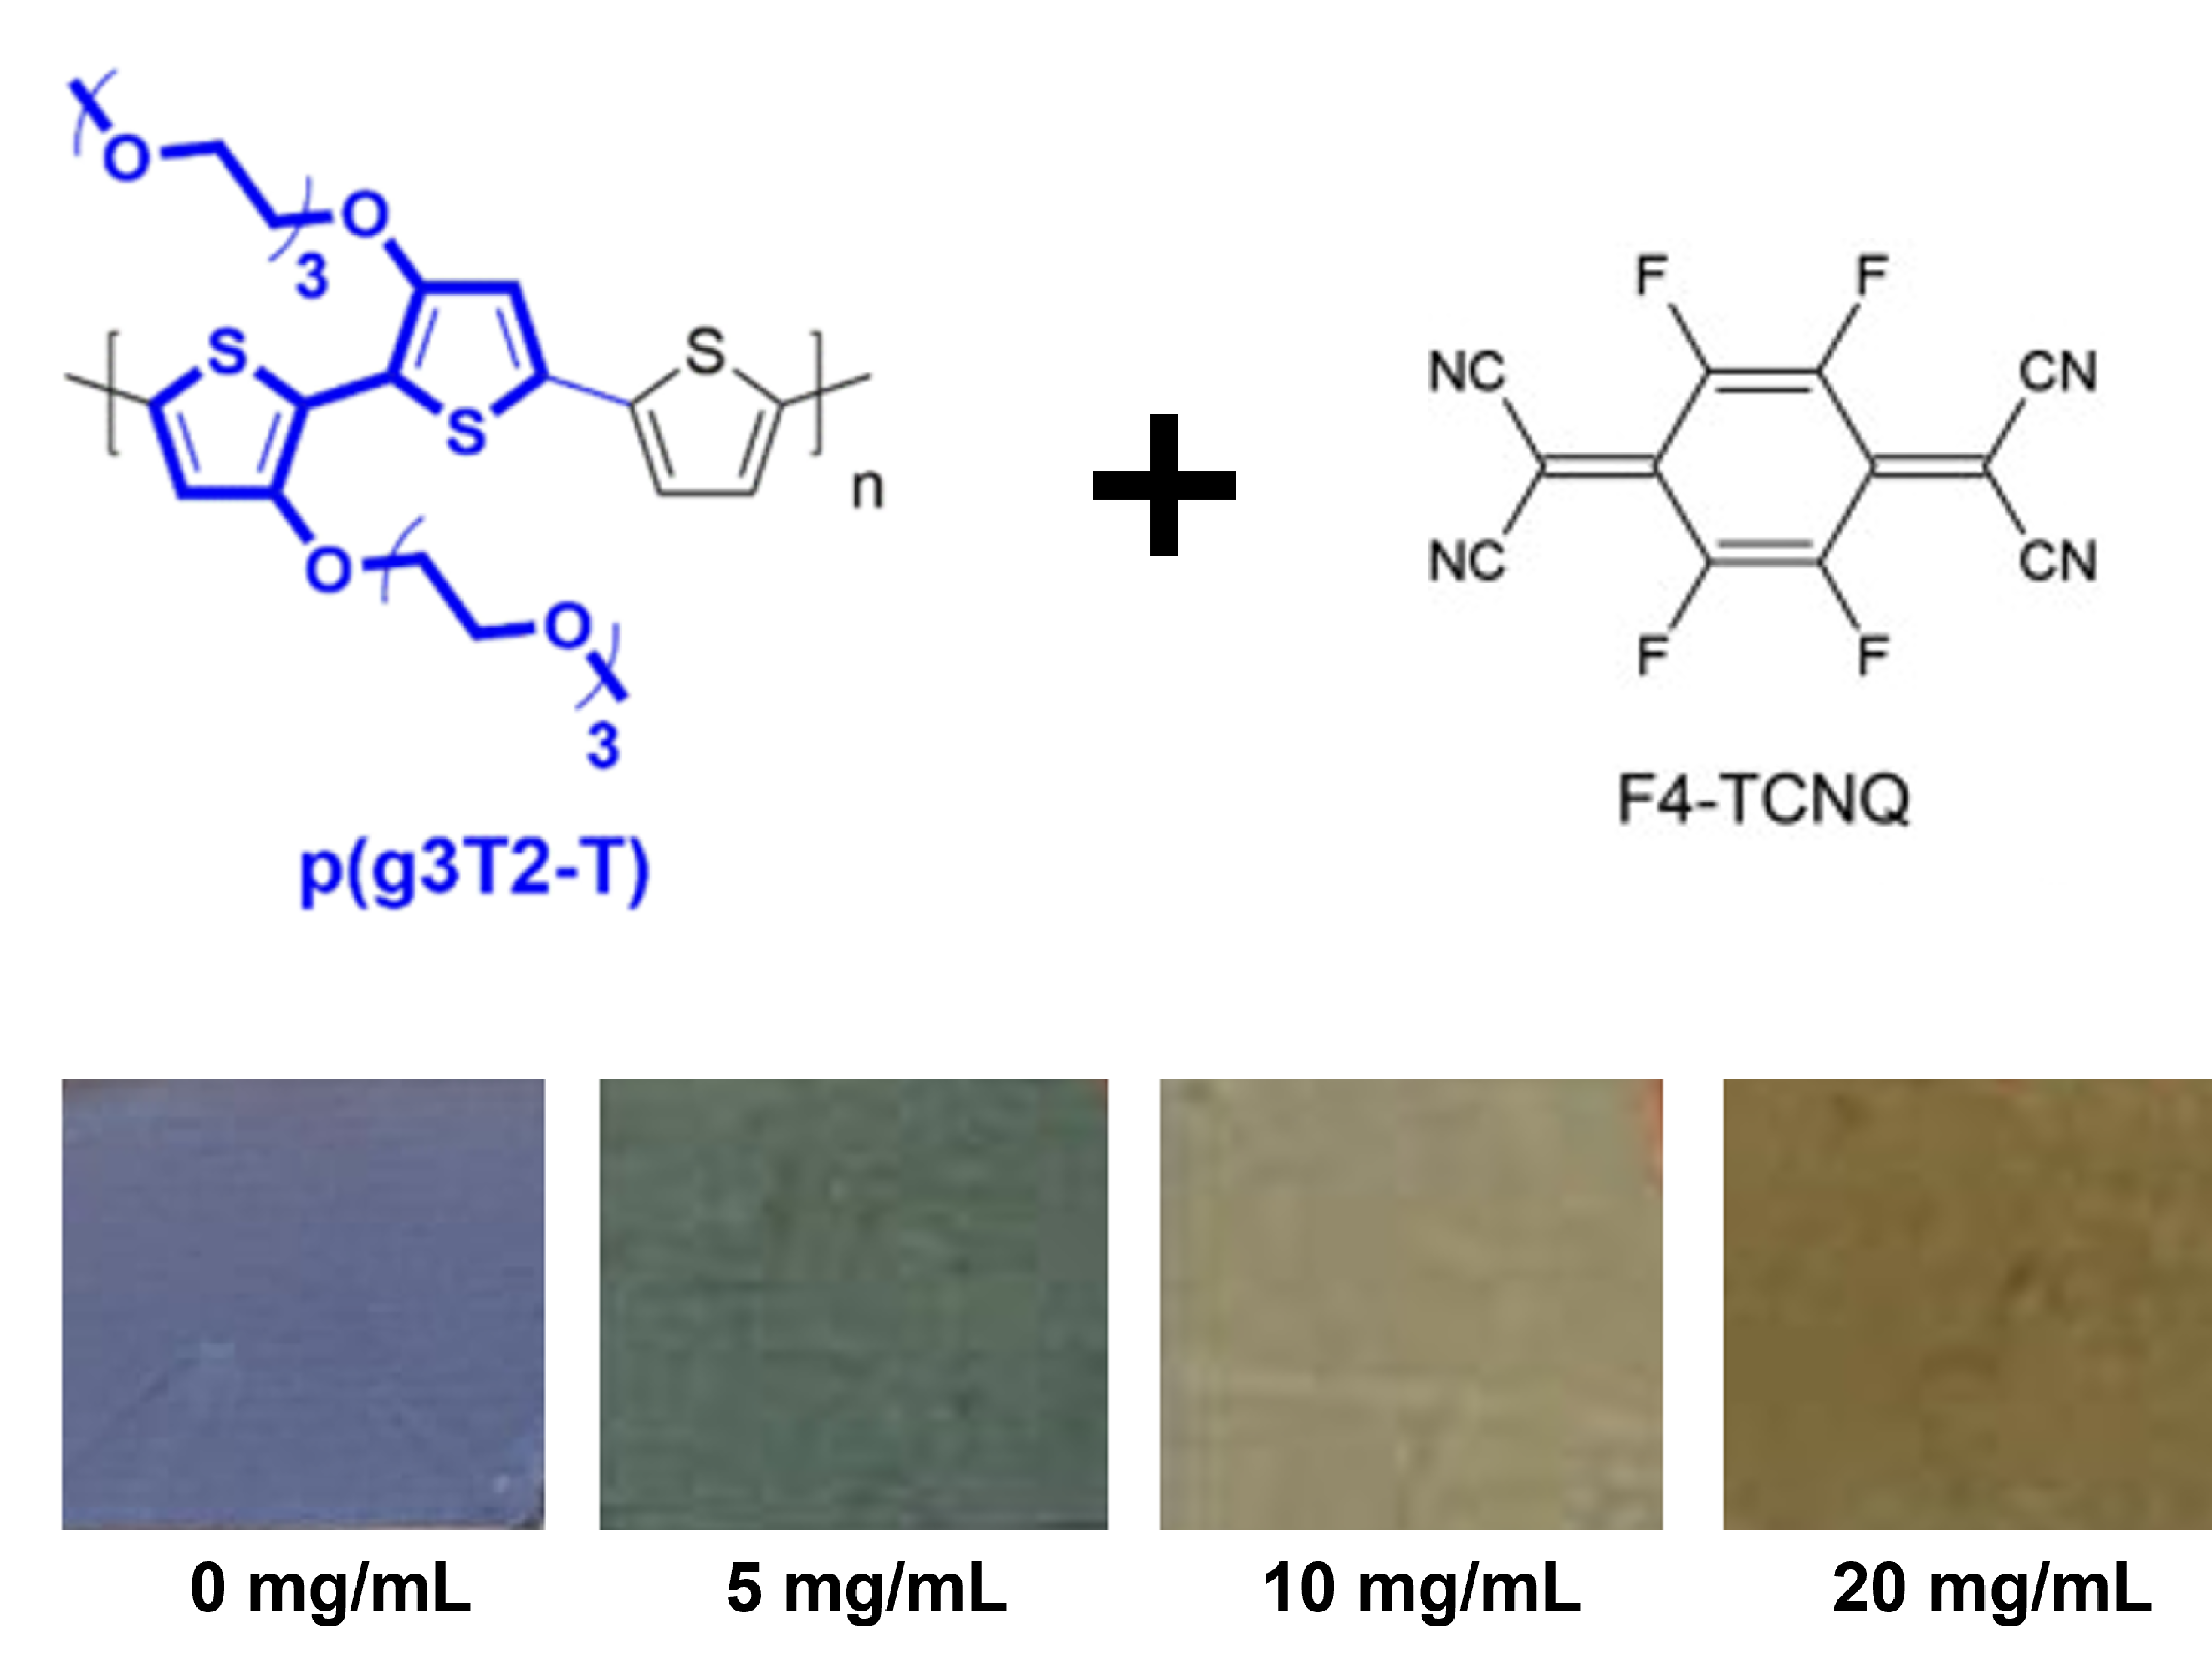
\includegraphics[width=7.5cm]{Images/pdf/doping_color.pdf}
  \caption[Color shift upon doping level increase]{Color change upon increasing dopant concentration from 0 to 20 mg/mL.
  \label{fig:color}}
\end{figure}

\subsection{Thickness, Sheet Resistance and Resistivity}

Sheet resistance and resistivity, as shown in Table \ref{tab:res}, were calculated using equations \ref{eq:rs} and \ref{eq:resist}, respectively, as described in previous chapter. The film thickness was determined through profilometer measurements, resulting in an approximate thickness of 70 nm.

\begin{table}[ht]
\centering
\caption{Sheet resistance and resistivity values for undoped and doped films of p(g3T2-T)}
\begin{tabular}{l|c|c|c|c}
& Undoped & 5 mg/mL & 10 mg/mL & 20 mg/mL \\\hline
R$_{S}$ ($\Omega$/sq) & 6.3M & 104.6k & 70.7k & 49.4k\\
$\rho$ ($\Omega$cm) & 44.1 & 0.73 & 0.49 & 0.35\\\hline
\end{tabular}
\label{tab:res}
\end{table}

Upon doping, a substantial decrease is observed in both sheet resistance and resistivity. However, this decrease is not as pronounced when higher dopant levels are introduced, as depicted in Figure \ref{fig:rho}. Nevertheless, when comparing the reduction among doped samples, a clear linear relationship becomes apparent with increasing the dopant concentration. 

\begin{figure}[ht]
  \centering
  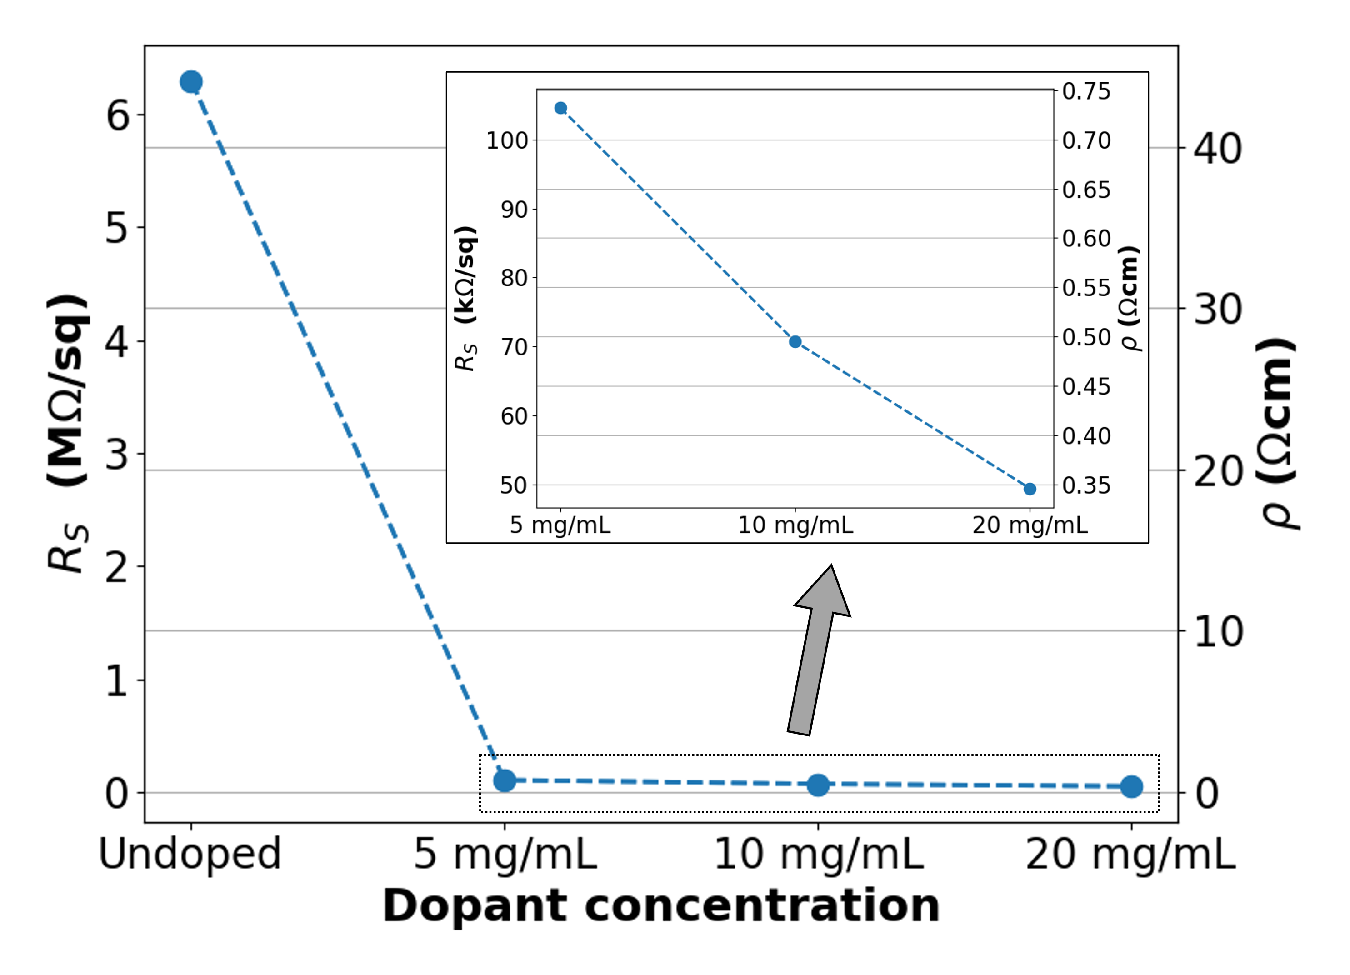
\includegraphics[width=7.5cm]{Images/pdf/resist+inlet.pdf}
  \caption[Sheet resistance and resistivity drop upon doping]{Sheet resistance and resistivity drop upon doping of p(g3T2-T). Inlet represents the quasi-linear drop of parameters as between doped samples.}
  \label{fig:rho}
\end{figure}

\subsection{Absorbance and Dopants Diffusion}
The visible color hue shift can be quasi-quantitatively described by examining the absorbance spectra of the samples, as illustrated in Figure \ref{fig:abs}. In the case of undoped-p(g3T2-T), there is a prominent absorption peak at 588 nm (red), which diminishes with increasing doping concentration, indicative of oxidation. Notably, new absorption peaks emerge at around 860 nm, a consequence of polaron generation, leading to new optical transitions, as explained in Chapter 2, Section \ref{subsec:moldop}. 

Tan et al. documented the appearance of new absorption peaks within the 300 to 600 nm range. The higher energy (lower wavelength) peak is generated by unreacted neutral dopant species (TCNQ$^{0}$), while the second is attributed to the new dopant anions (TCNQ$^{-}$), which induce charges in our polymer \cite{tanTuningOrganicElectrochemical2022}. Additionally, it is worth noting that, after several days of storage, the initially dominant peak of unreacted neutral dopants diminishes in intensity relative to the anions peak. This observation suggests ongoing diffusion of dopants through the polymer over time. 

\begin{figure}[ht]
  \centering
  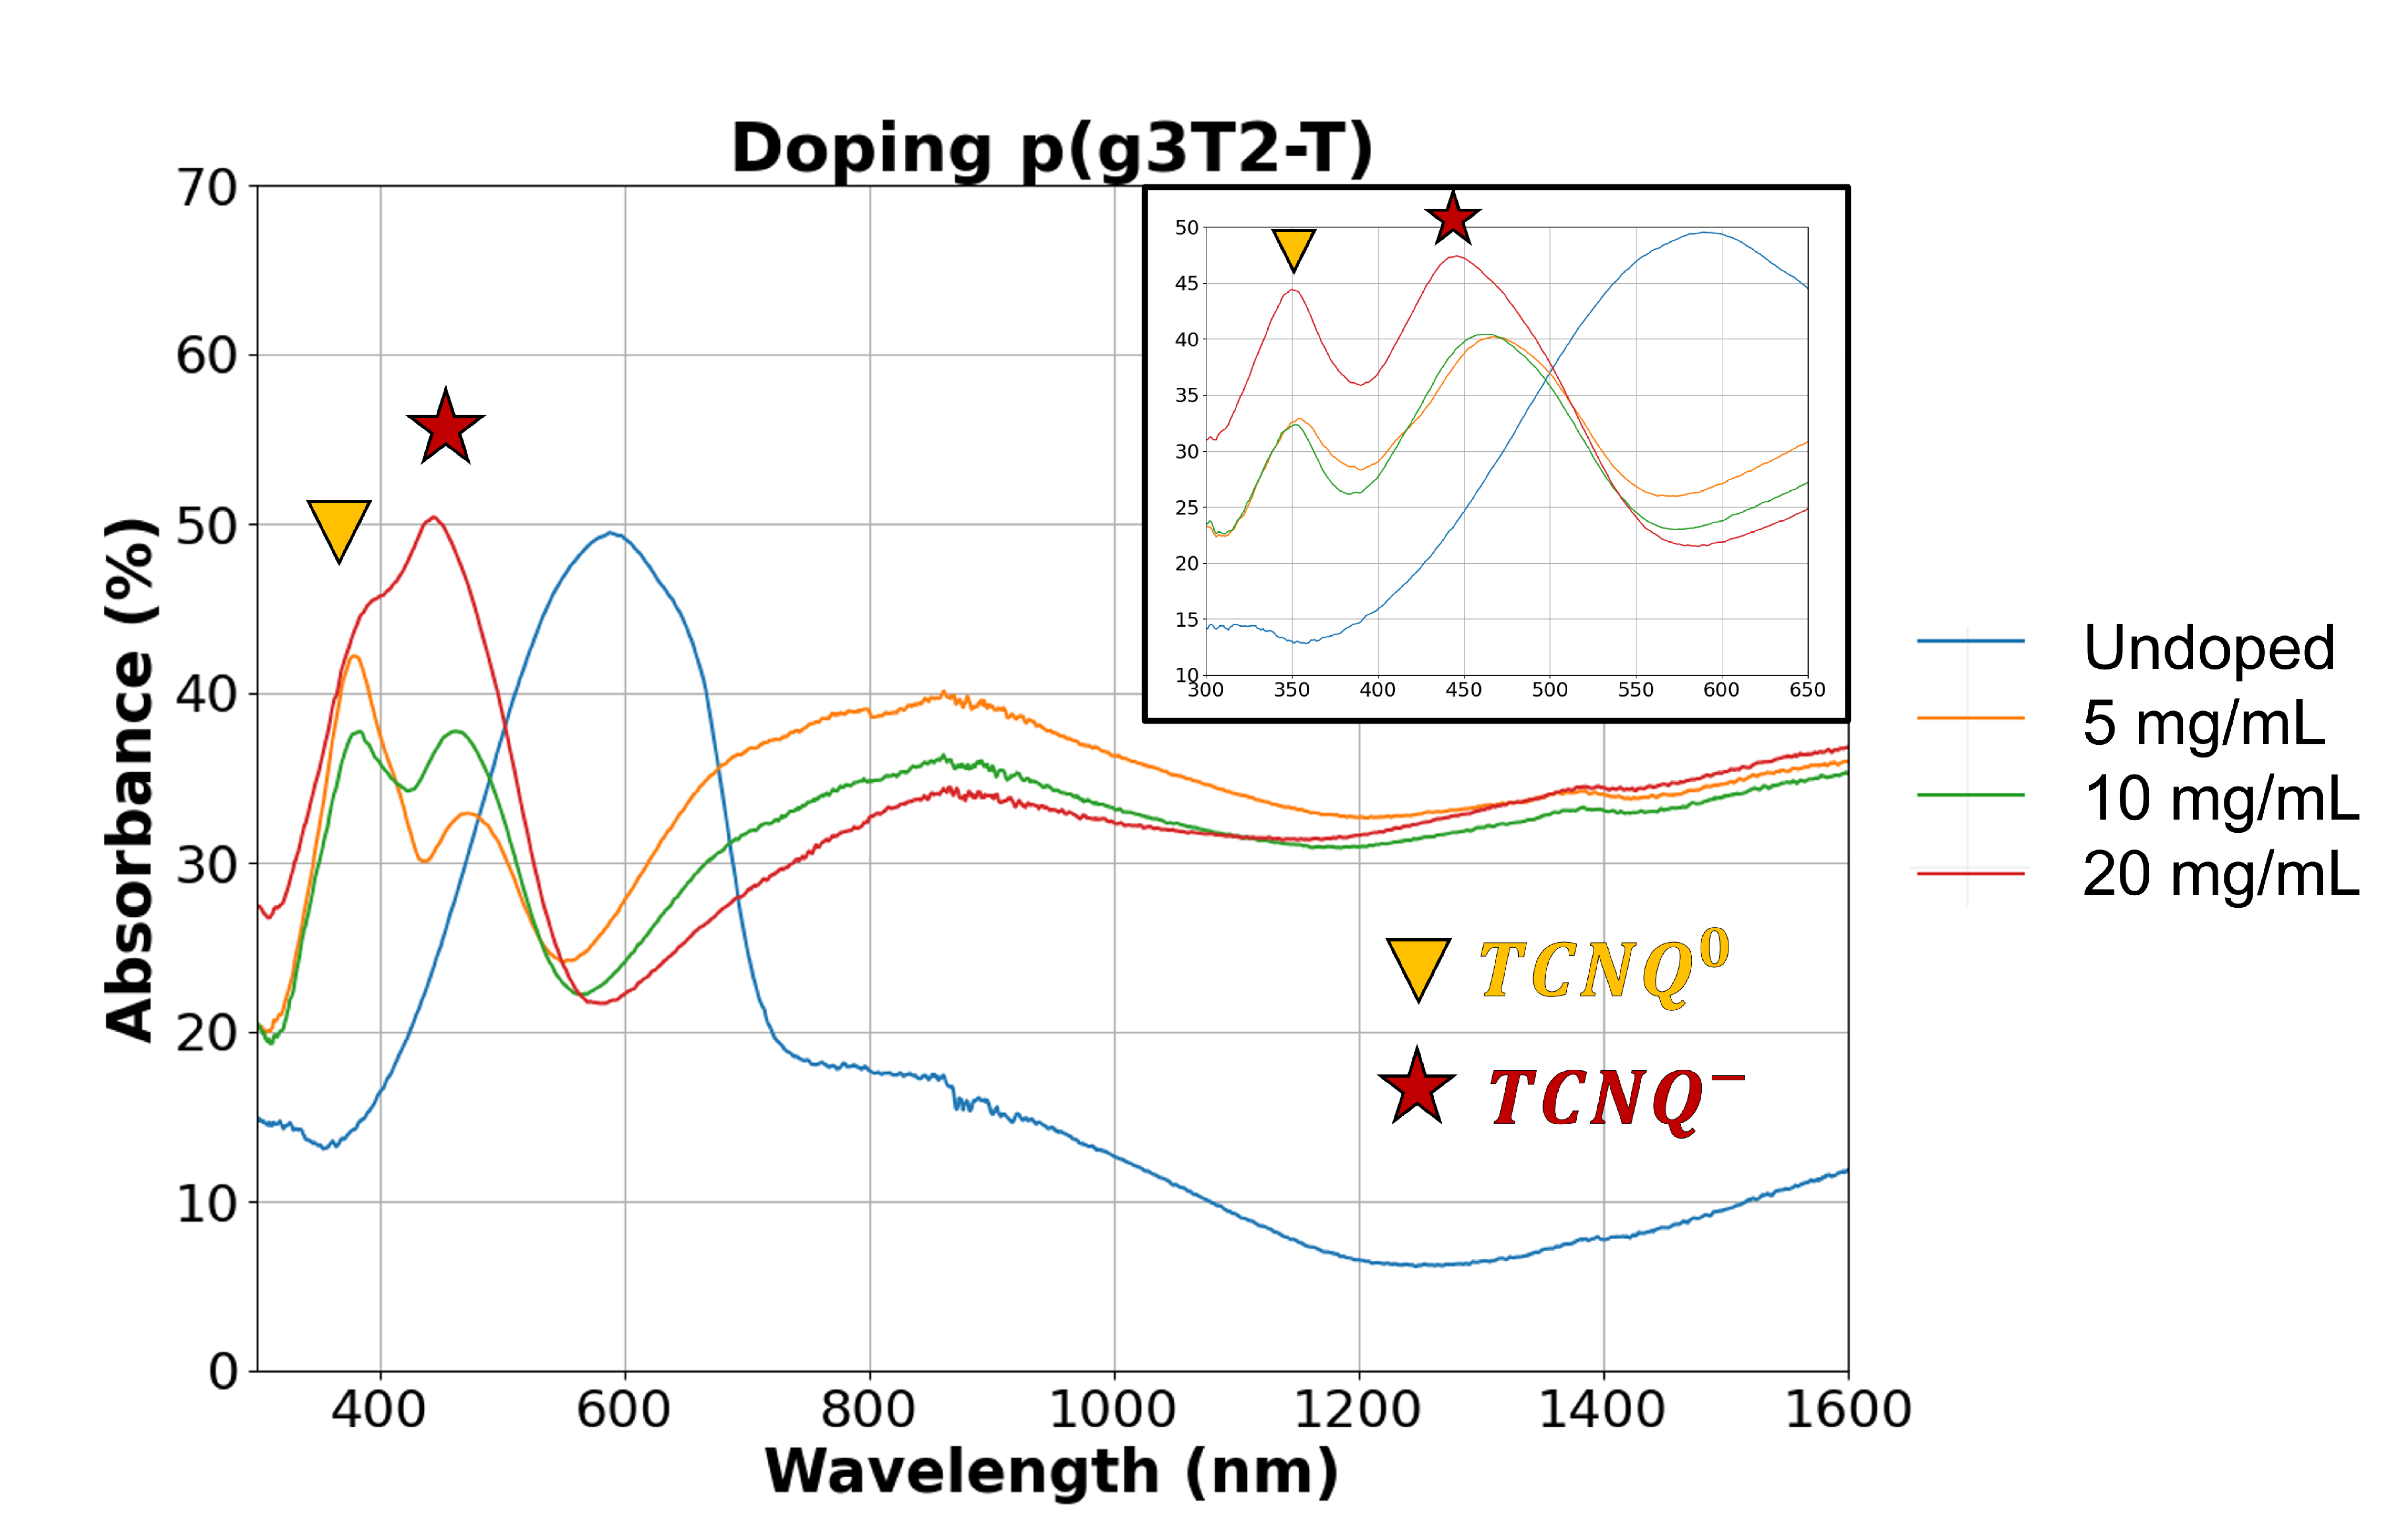
\includegraphics[width=10cm]{Images/pdf/abs+inlet.pdf}
  \caption[Absorbance spectra of different doping levels of p(g3T2-T)]{Spectra of undoped and doped-p(g3T2-T) at different doping levels, corresponding to samples on Figure \ref{fig:color}. Inlet represents absorbance after two weeks of storage in ambient conditions.}
  \label{fig:abs}
\end{figure}

Absorbance values are directly correlated with the density of states of these new optical transitions \cite{bredasPolaronsBipolaronsSolitons1985}. In our spectra, the absorbance value at 860 nm of the lowest-doped p(g3T2-T) sample (5 mg/mL) is relatively higher, around 40\%. This might initially appear counterintuitive. However, as the doping concentration increases, the formation of bipolarons and bipolaron bands becomes energetically more favorable \cite{enenglDopinginducedAbsorptionBands2016} . This phenomenon aligns with observations in the higher wavelengths, such as at 1600 nm, where absorbance increases in the more highly doped p(g3T2-T) sample.

Moreover, Tan et al. reported the formation of bipolaron in this specific context, evidenced by a shift to lower energies in the broad absorbance spectrum within the mid-IR region (wavenumbers 1000-1600 cm$^{-1}$) \cite{tanTuningOrganicElectrochemical2022}. Consequently, further analysis of hole bipolaron formation can be conducted with Fourier Transform InfraRed (FTIR) spectroscopy.
 
\subsection{Workfunction}

In the context of studying electron energy levels with UPS, the ideal film preparation involves working under inert conditions to prevent contamination. However, our current OECT fabrication process unavoidably exposes our films to ambient conditions. Consequently, we conducted measurements following deposition under these ambient conditions. As expected, we observed an increase in the workfunction, as evidenced by a shift in the Fermi level of the polymer. This shift towards the HOMO level becomes more pronounced at higher dopant concentrations, as depicted in Figure \ref{fig:ups}, which is characteristic of p-type doping. Unfortunately, potential contamination issues prevented the measurement of samples with a dopant concentration of 20 mg/mL, but the trend is clearly discernable.

\begin{table}[ht]
\centering
\caption{Calculated workfunction from UPS measurements and represented in Figure \ref{fig:ups}.}
\begin{tabular}{l|c|c|c}
& Undoped & 5 mg/mL & 10 mg/mL \\\hline
E$_{HBEC}$ [eV] & 17.35 & 16.47 & 16.36\\
E$_{HOMO}$ (vs E$_{F}$) & 4.28 & 3.27 & 3.24\\
WF [eV] & 3.87 & 4.28 & 4.86\\\hline
\end{tabular}
\label{tab:ups}
\end{table}

It is crucial to recognize that UPS is a surface-sensitive measurement. The penetration depth of the ultraviolet-range photons in UPS is limited to approximately 2 nm, significantly less than the thickness of our polymer film (approximately 70 nm). Consequently, this technique restricts our understanding of the diffusion of dopants throughout the entire volume of the polymer. Although, we gained some insights into this matter in the previous subsection, further analysis could be carried out using X-Ray Photoelectron Spectroscopy, which offers a depth profiling mode. %but along with depth profiling mode 3

\begin{figure}[ht]
	\centering
	\subfloat[]{{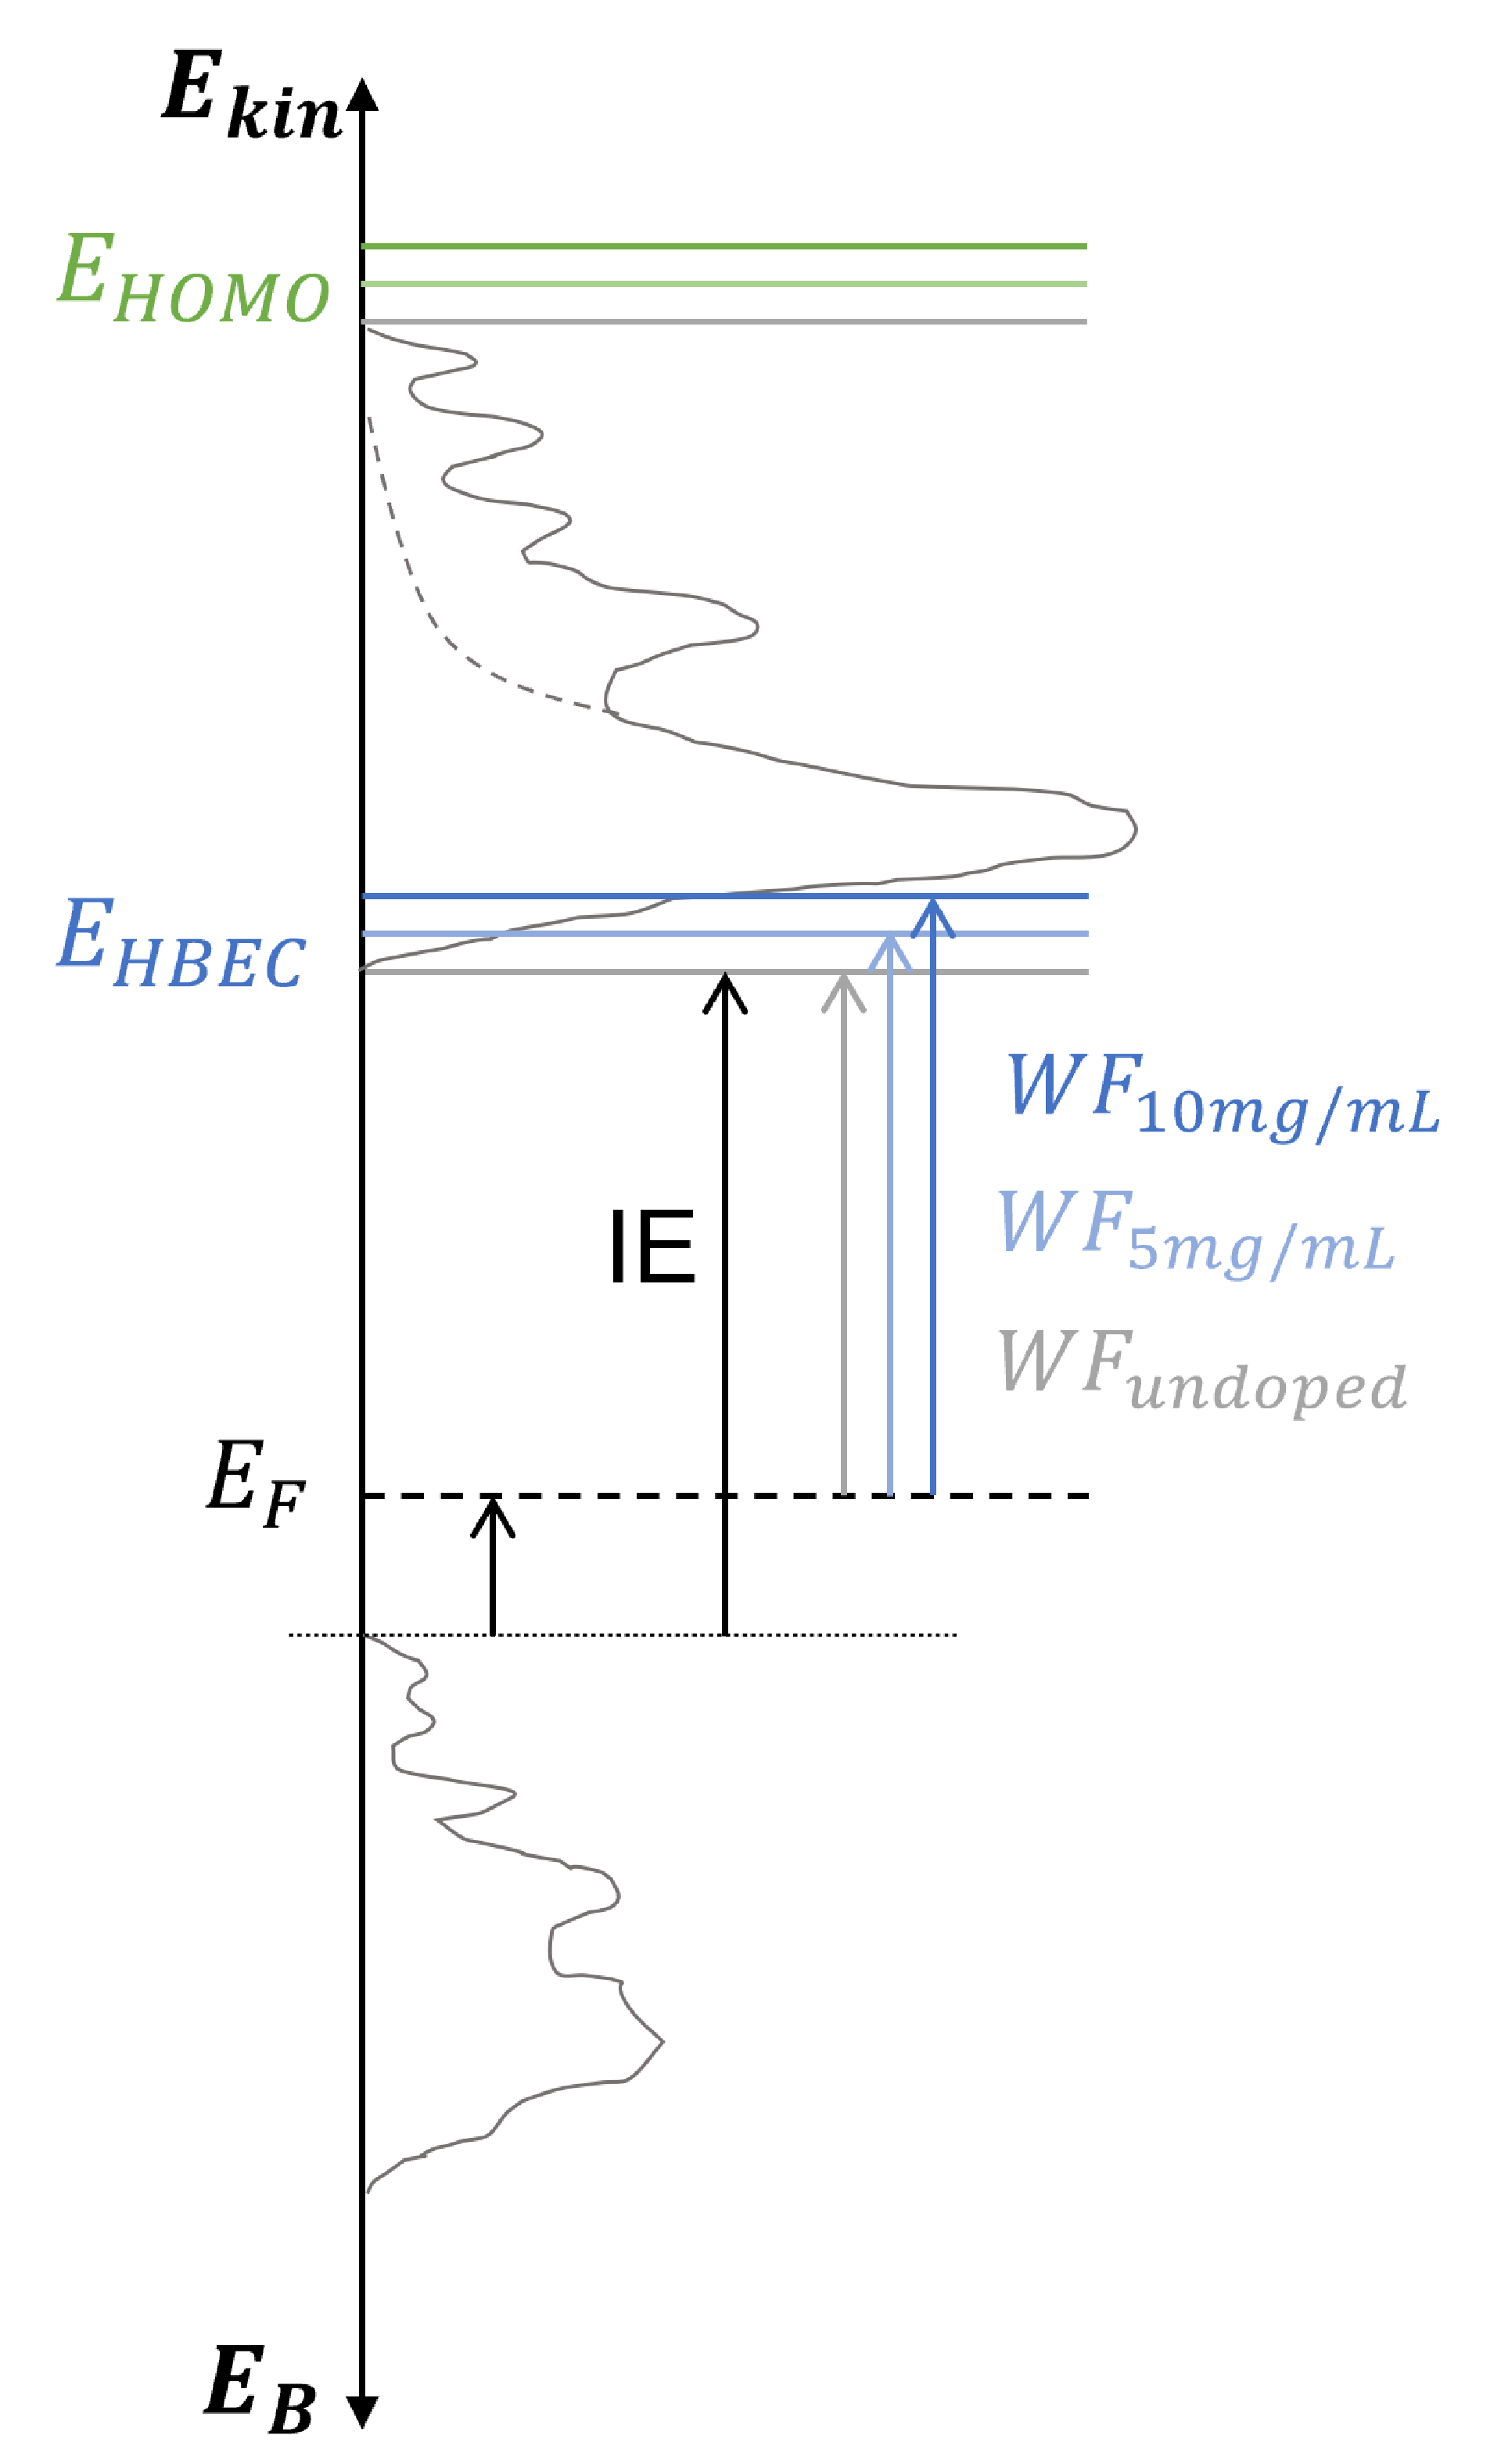
\includegraphics[width=6cm]{Images/pdf/WF_final.pdf} }}
	%\qquad
	\hspace{2em}
	\subfloat[]{{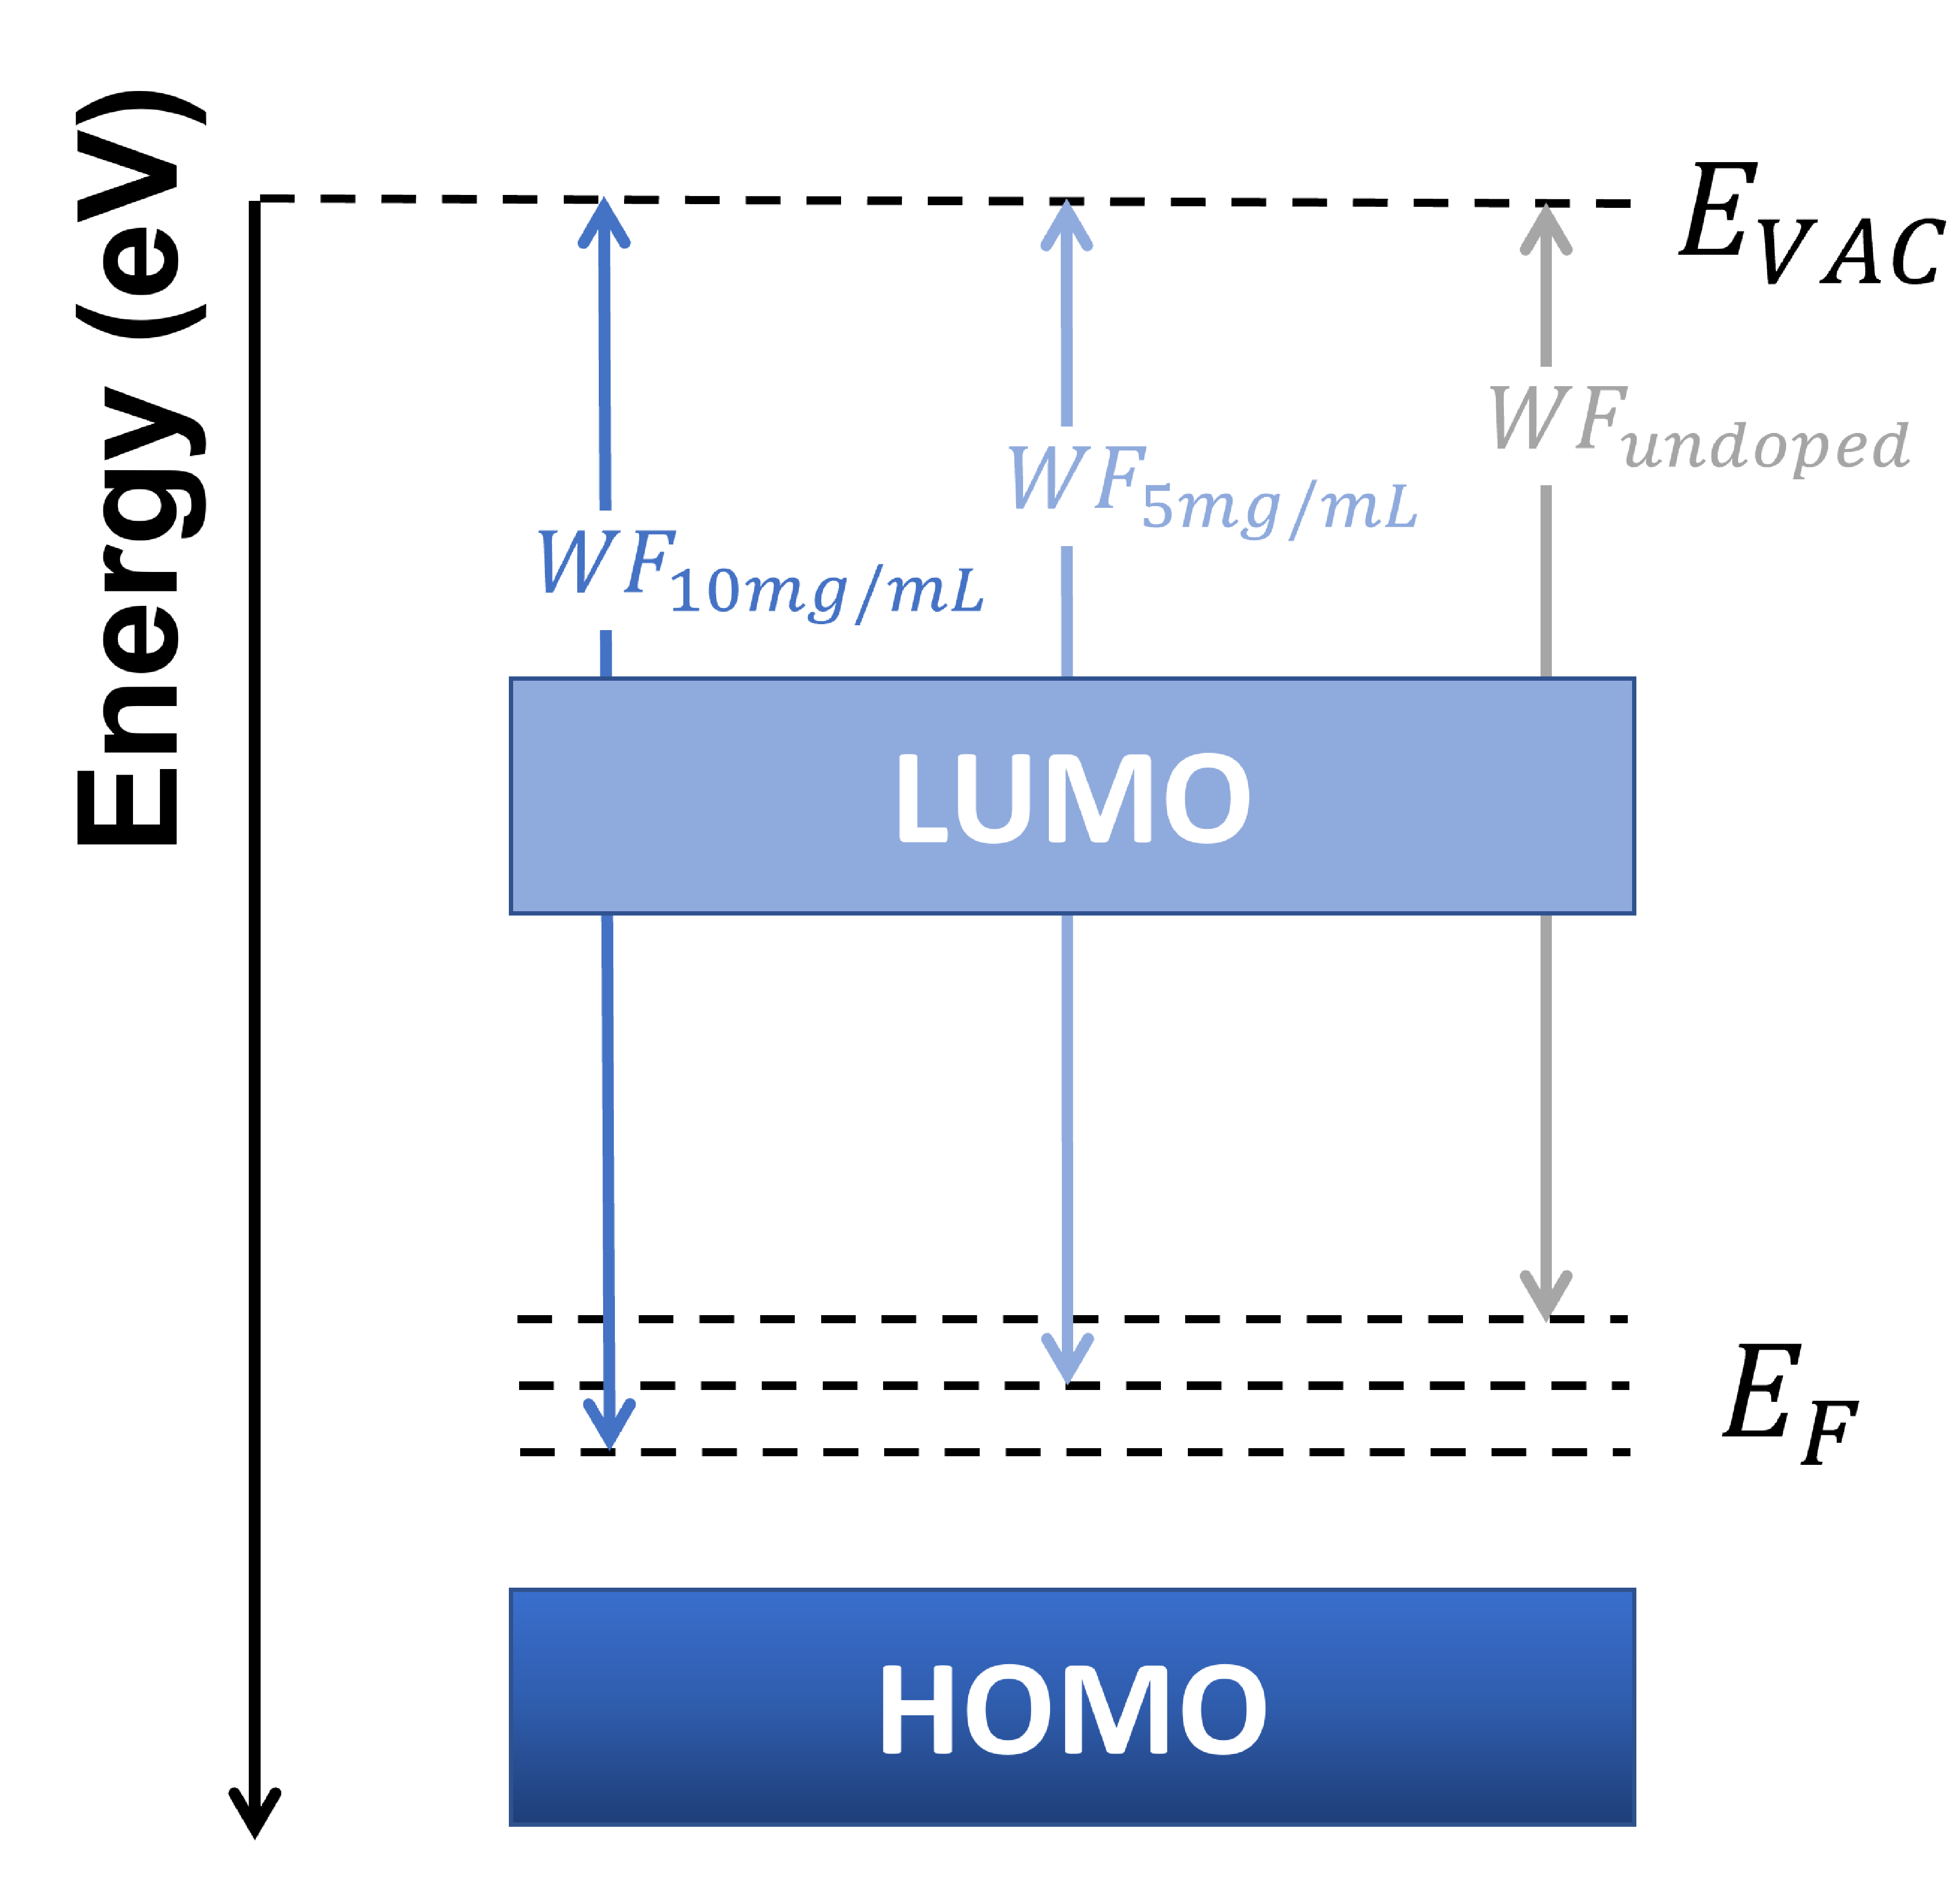
\includegraphics[width=6cm]{Images/pdf/WF.pdf} }}
	\caption[Representation of the Fermi level shift upon doping]{ Graphical representation of A) the relationship between the binding energies E$_{B}$ and the kinetic energy of the photoelectrons E$_{kin}$, and B) the Fermi level shift, upon doping.} 
	\label{fig:ups}
\end{figure}

%\subsection{Roughness}

\section{Fabrication of Organic Electrochemical Transistors}
The patterning process was successfully accomplished via photolithography, as detailed in Section {subsec:oect}, employing a mask that included a microstructure gate. This setup is ideal for studying OECTs with both channel and gate constructed from the same OMIEC material, commonly PEDOT:PSS. The result of this process is displayed in Figure \ref{fig:channel}. 

\begin{figure}[ht]
  \centering
  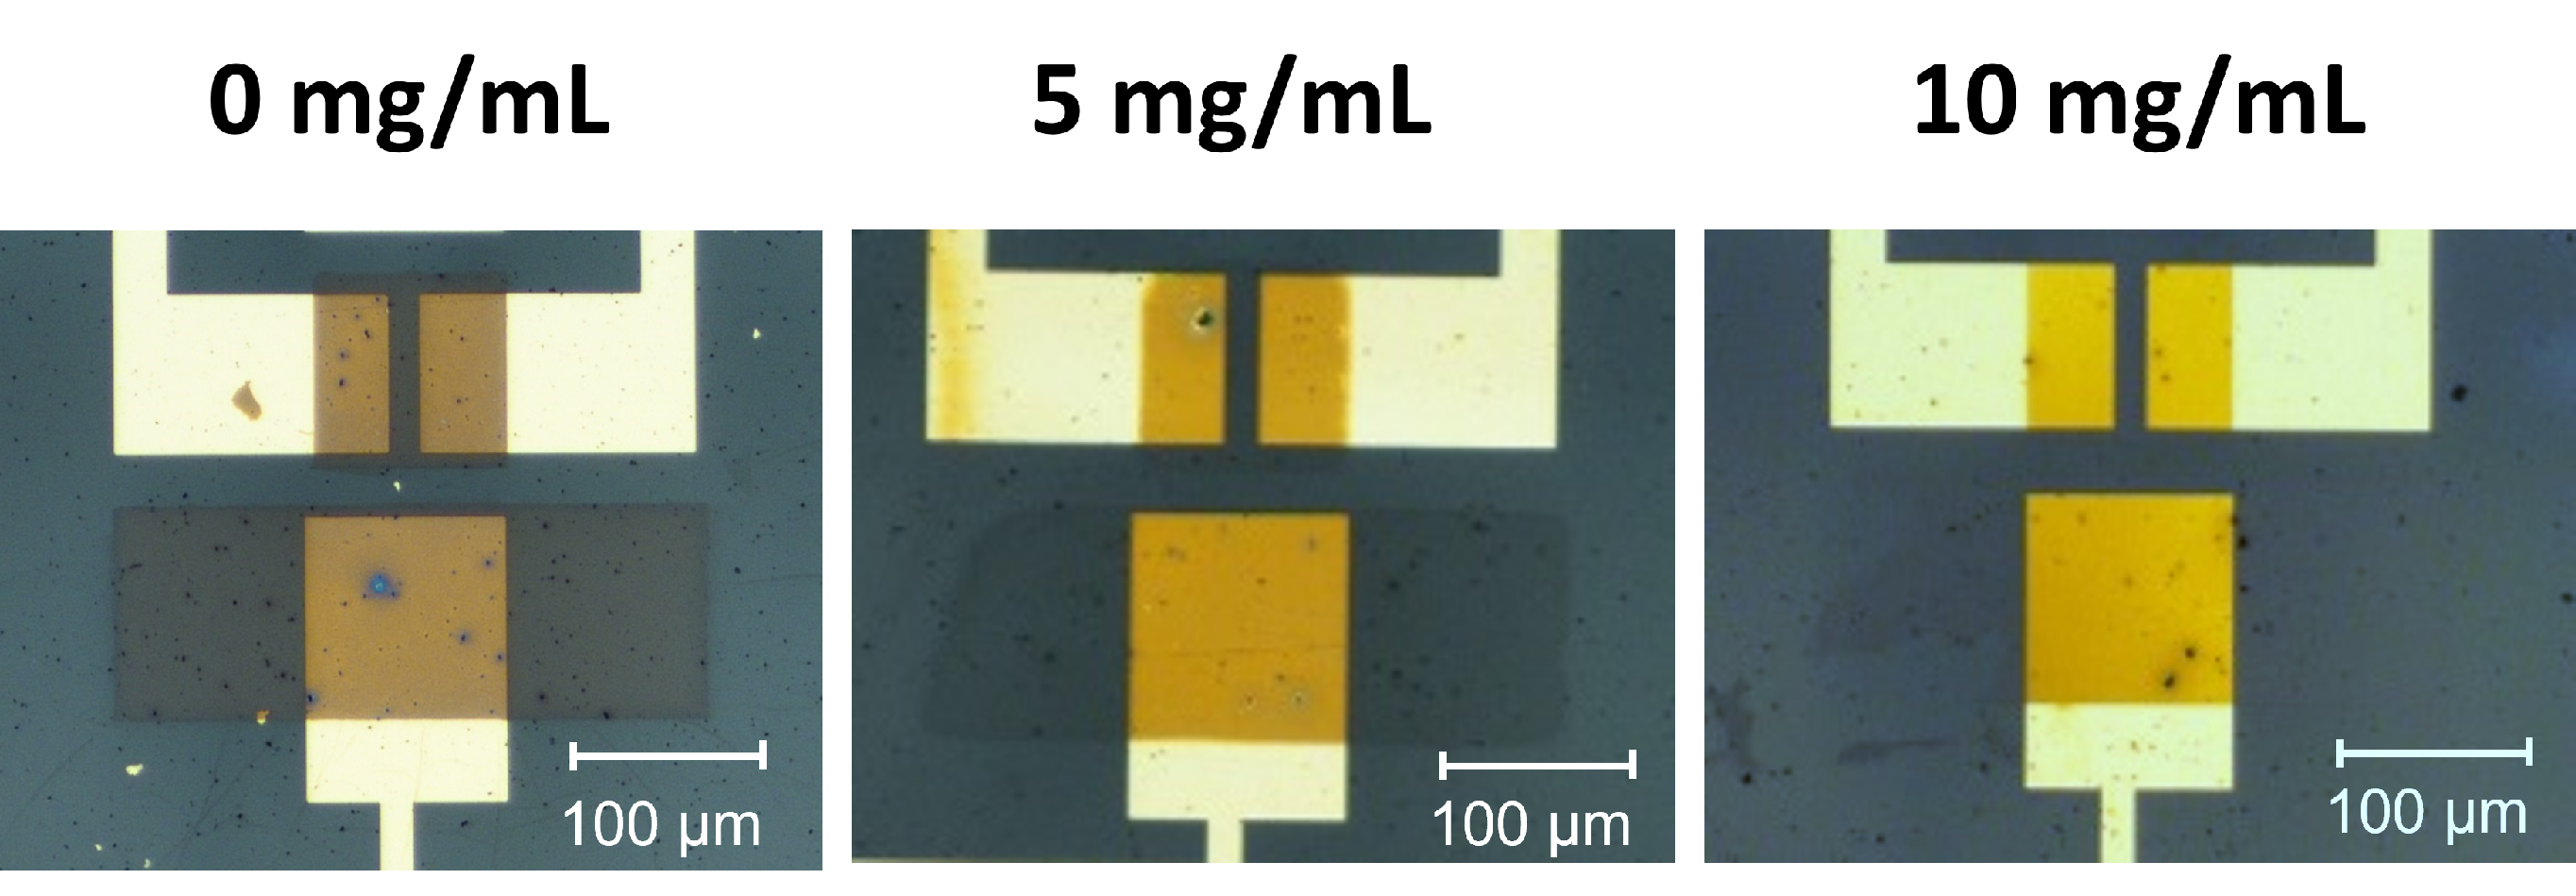
\includegraphics[width=10cm]{Images/pdf/BigGateDevices.pdf}
  \caption[Micrographs of a patterned channel and gate p(g3T2-T) at different doping levels]{Micrographs of patterned channel and gate with p(g3T2-T) undoped, 5 mg/mL and 10 mg/mL dopants, following procedures explained in Section \ref{subsec:channel}.}
  \label{fig:channel}
\end{figure}

%Prior biasing gate, which is due to passive (ion) diffusion?

\subsection{Influence of Doping on OECT Channel}
Our ultimate goal is to study fully patterned solid-state OECTs that will enable integrated circuits (IC). To achieve this, it was imperative to initially investigate the isolated impact of channel doping on our devices. Several hypothesis were formulated, based on reference \cite{tanTuningOrganicElectrochemical2022}:

\begin{enumerate}
\item Modifying channel doping may negatively impact transfer characteristics.
\item The introduction of ionic species (TCNQ$^{-}$) into p(g3T2-T) should result in depletion-mode devices with positive threshold voltages. This is because a higher positive gate bias would be needed to counteract these anions and turn off the device.
\end{enumerate}

As explained in the previous chapter, we paired our channel with a non-polarizable gate such as a Ag/AgCl, a widely used configuration for investigating OECT-based materials, and coupled it with a SSE precursor. Unfortunately, the sample that used a solution with A dopant concentration of 20 mg/mL exhibited issues with doping homogeneity. While photolithography was still feasible, it could not provide a fair basis for comparison with the other devices. Consequently, this sample will be excluded from our analysis.

The results shown in Figure \ref{fig:transx2}, Figure \ref{fig:shift1} and Figure \ref{fig:vth_vds} correspond to the same device and the same loop on each sample (undoped, 5 mg/mL, and 10 mg/mL dopants) from the same batch of materials. After reporting these findings on the analysis of individual devices, a more comprenhesive statistical study will be conducted on operational devices from each sample. 

It is essential to note that for the statistical analysis of this section, despite our efforts to increase the yields, only 3 or 4 out of the 14 devices were operational on each sample. Further improvements in the photolithograpy process were necessary and accomplished, and will be detailed in subsequent sections of this chapter. 

Transfer characteristics are illustrated in Figure \ref{fig:transx2}A, C, E, corresponding to undoped, 5 mg/mL, and 10 mg/mL dopants, respectively. Notably, a positive turn-on voltage is observed in the undoped OECT device, indicating the rapid oxidation (unwanted doping) of p(g3T2-T) under environmental conditions due to its low ionization potential (IP). 

The drain current ($I_{D}$) of the undoped device exhibits higher values than doped devices, Hidalgo et al.  \cite{hidalgocastilloSimultaneousPerformanceStability2022a} reported that pristine p(g3T2-T) exhibits oxygen reduction reaction activity in oxygen-saturated conditions, resulting in an increase in current within the polymer until saturation. To address this issue, it will be necessary to control the oxidation state of the polymer during selective steps of the fabrication process or fin a way to reverse the oxidation of p(g3T2-T), which will be explored in subsequent sections.

Gate current ($I_{G}$) is represented by dotted lines, and it is apparent that the drain OFF current ($I_{D,OFF}$) is dominated by this leakage current in all devices. %Figure \ref{fig:shift1} shows that doped devices exhibit minimal differences in $I_{D,OFF}$.

Notably, the device with the highest dopant concentration (10 mg/mL dopant) shows signs of breakage as $V_{DS}$ becomes more negative (Figure \ref{fig:transx2}E and Figure \ref{fig:shift1}D). Consequently, this measurement will be exclueded from the calculation of transconductance and threshold voltage.

\begin{figure}[!htb]
    \centering
    \subfloat[Undoped device]{{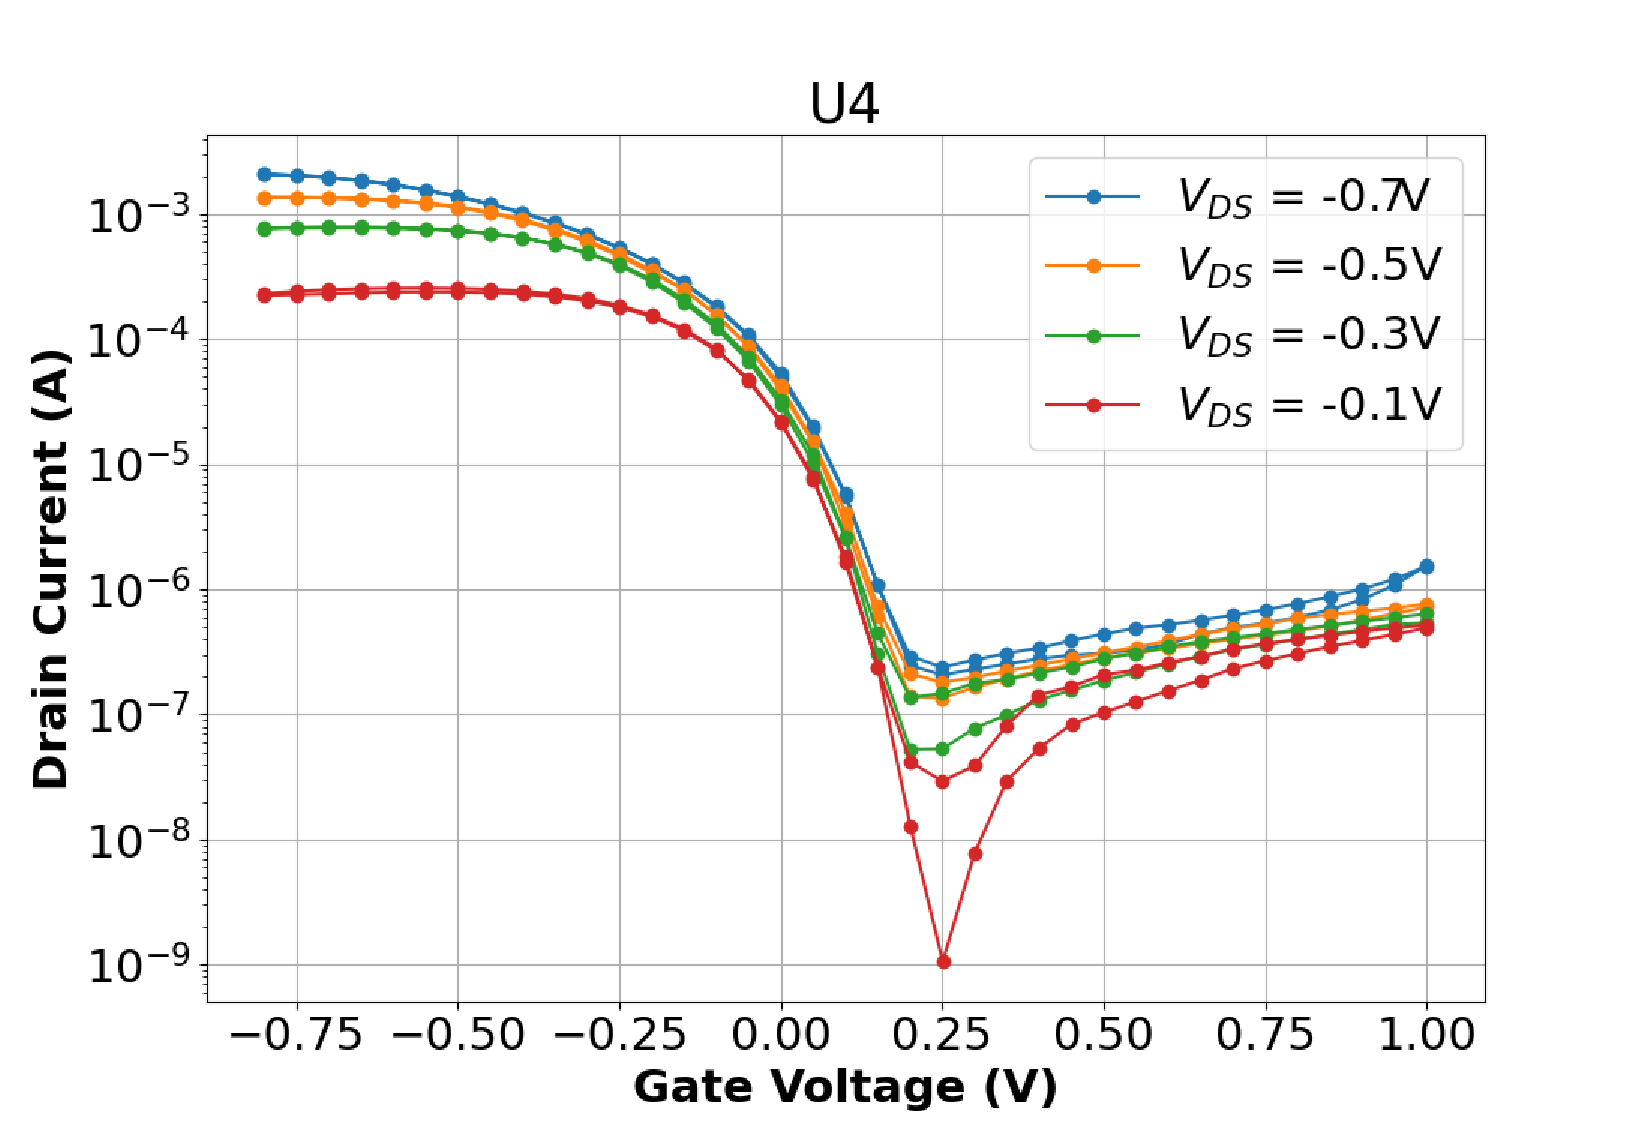
\includegraphics[width=5.7cm]{Images/pdf/transfer_undoped.pdf} }}
    \subfloat[Undoped device]{{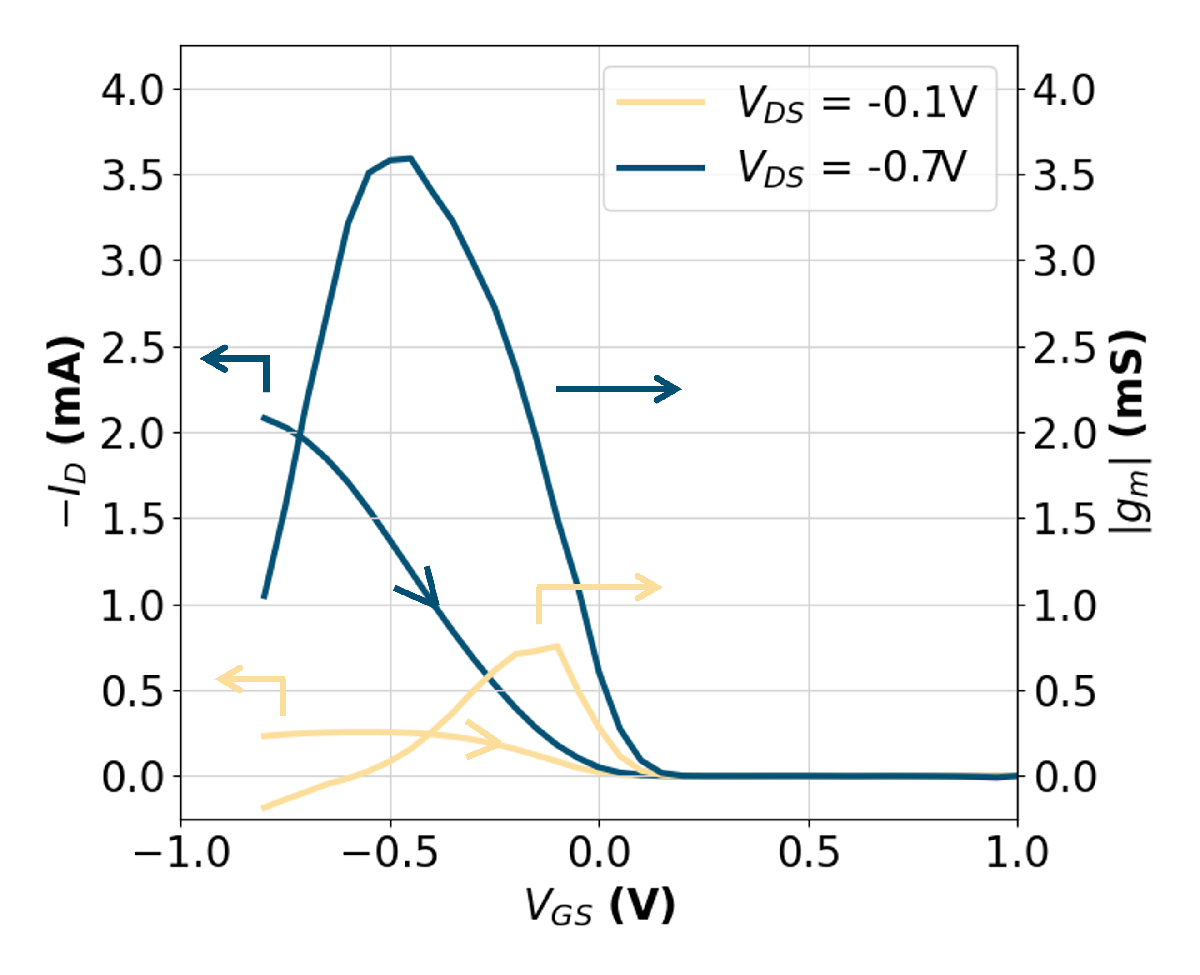
\includegraphics[width=5.3cm]{Images/pdf/id+gm_undoped_final.pdf} }}
    \qquad
    \subfloat[5 mg/mL dopant device]{{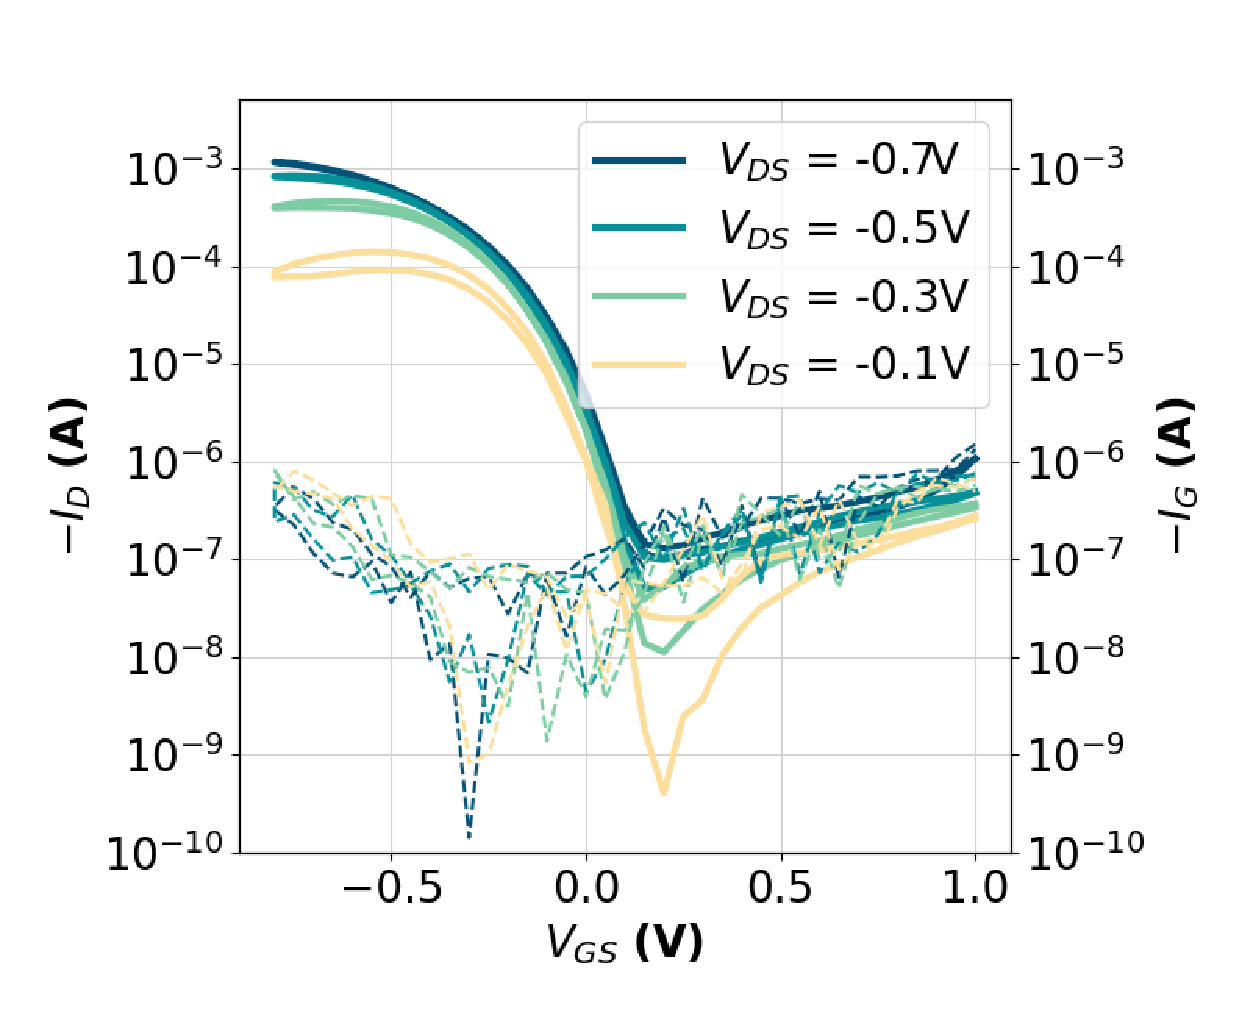
\includegraphics[width=5.7cm]{Images/pdf/transfer_doped5.pdf} }}
    \subfloat[5 mg/mL dopant device]{{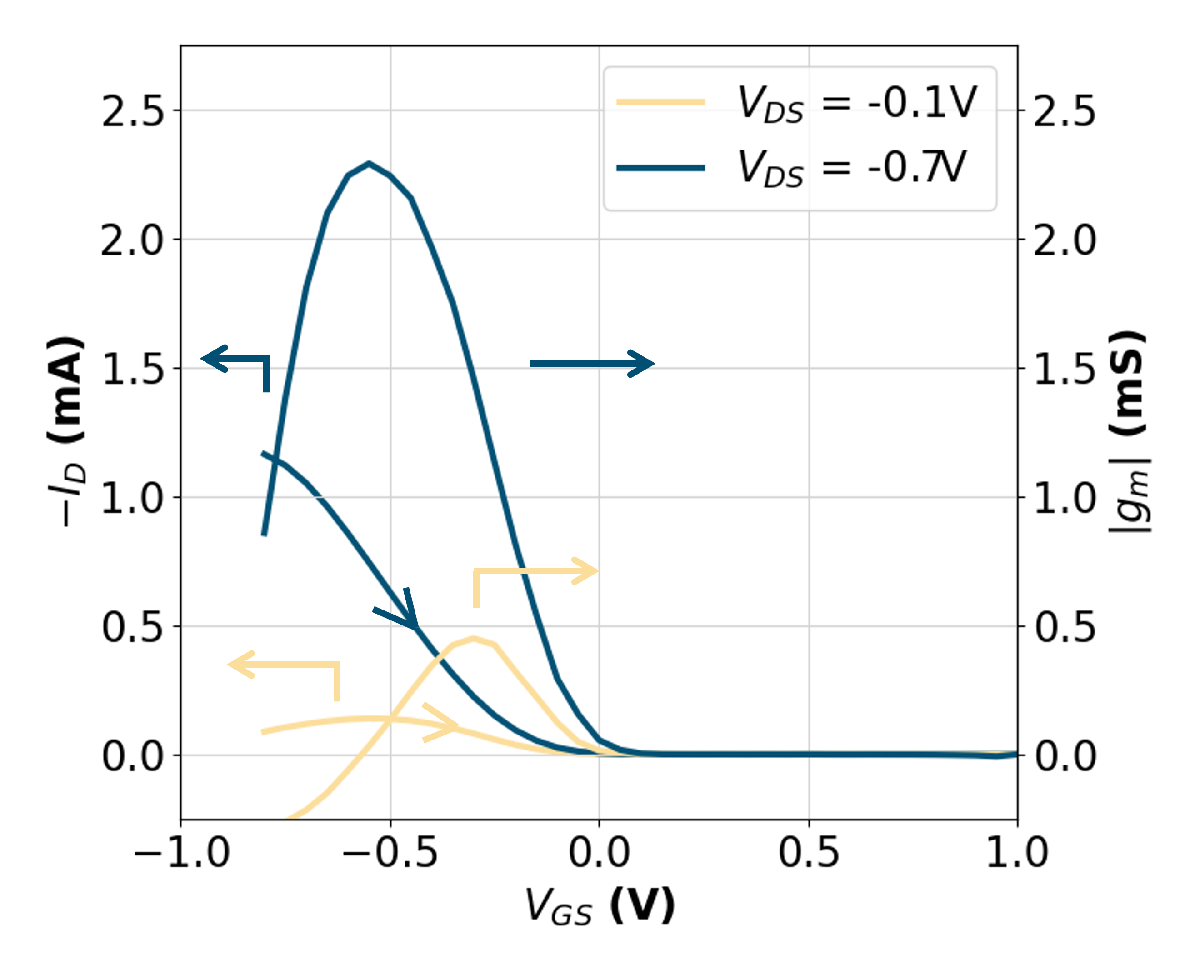
\includegraphics[width=5.3cm]{Images/pdf/id+gm_doped5_final.pdf} }}
    \qquad
    \subfloat[10 mg/mL dopant device]{{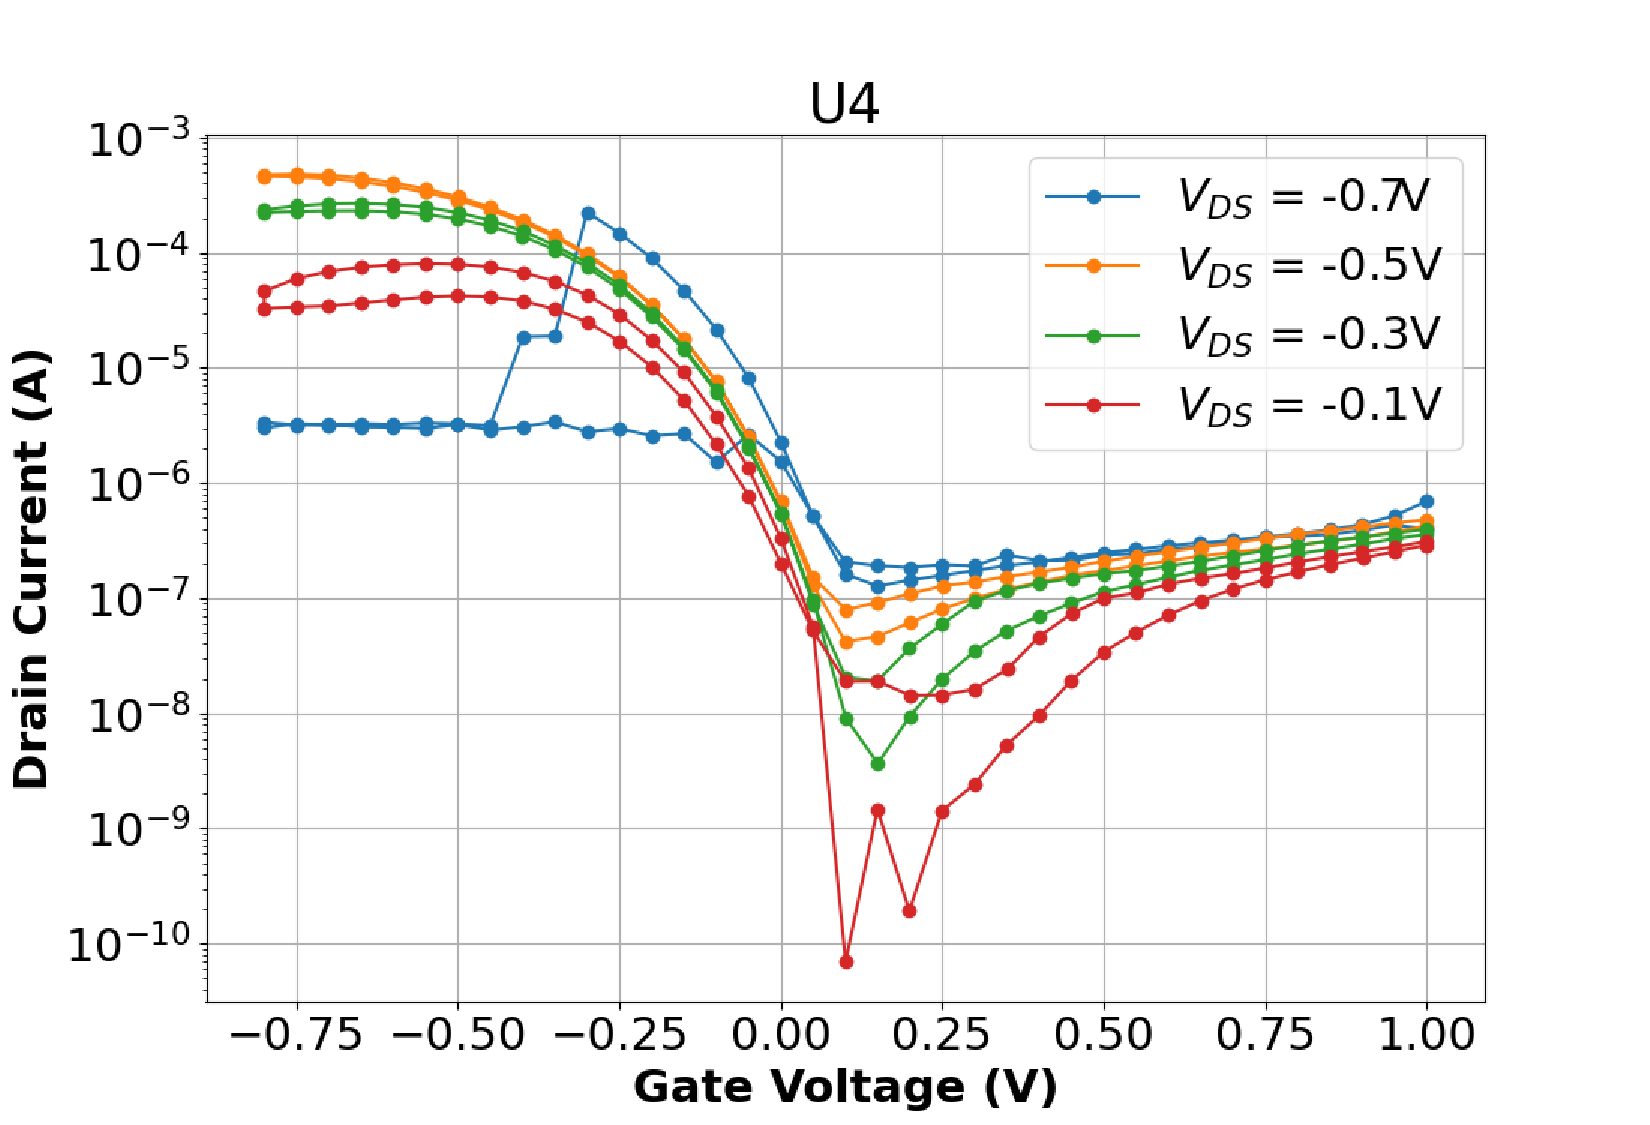
\includegraphics[width=5.7cm]{Images/pdf/transfer_doped10.pdf} }}
    \subfloat[10 mg/mL dopant device]{{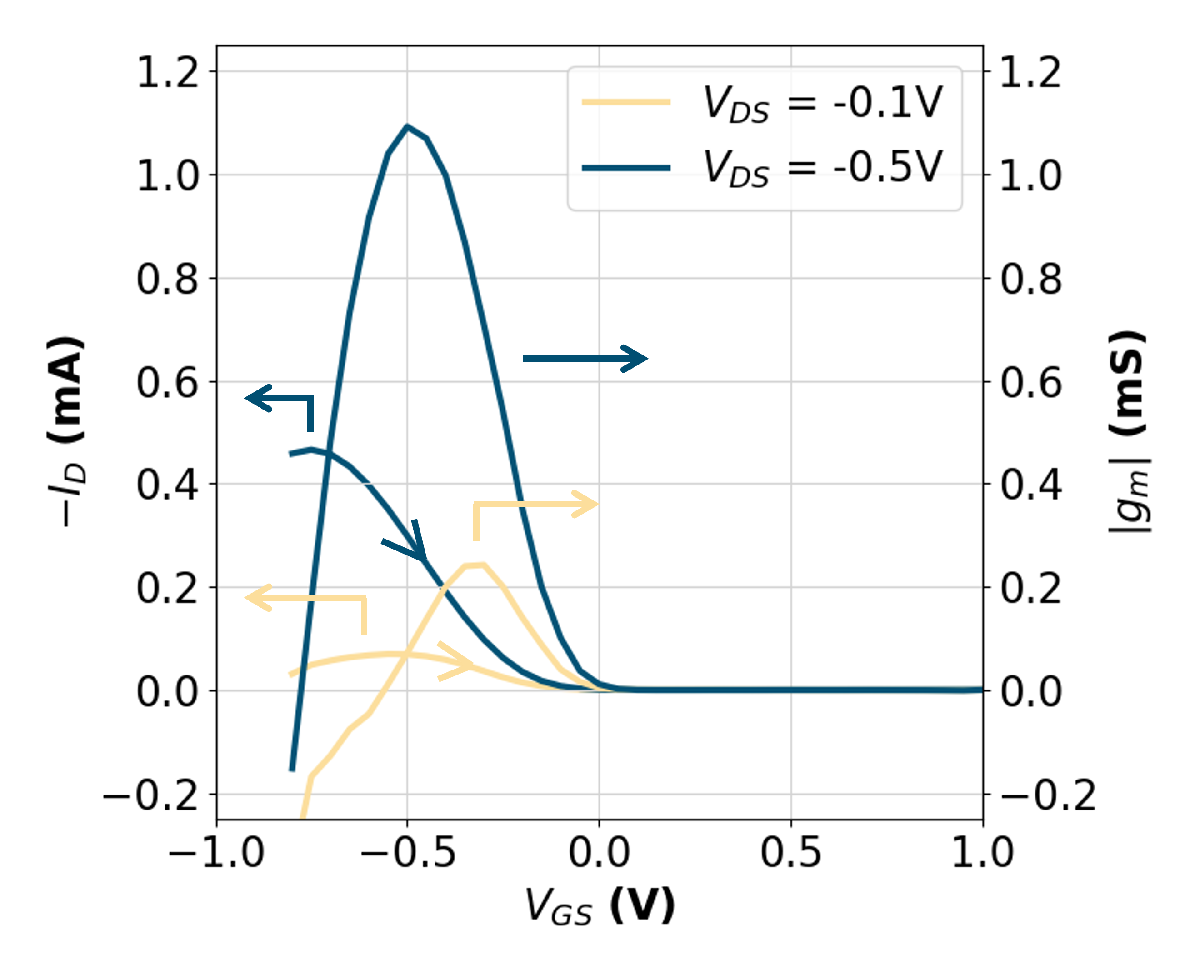
\includegraphics[width=5.3cm]{Images/pdf/id+gm_doped10_final.pdf} }}
    \caption[Transfer characteristics and transconductance at different doping levels and $V_{DS}$]{A), C), E) Transfer characteristics of all measured $V_{DS}$ including the gate leakage current $I_{G}$ B), D), F) Transfer curves (off-switching) with corresponding transconductance. Each group of graphs for undoped, 5 mg/mL and 10 mg/mL doped p(g3T2-T) channel, respectively.}
    \label{fig:transx2}
\end{figure}

%U4 loop 2 as undoped pattern
%U2 loop 3 for doped 5
%U4 loop 3 for doped 10

Figure \ref{fig:shift1} illustrates that doped devices exhibit minimal differences in $I_{D,OFF}$ but  there is a noticeable decrease in $I_{D,ON}$ as the doping levels increase. This is reflected in the maximum transconductance values displayed in Table \ref{tab:trans}, where a clear drop of |$g_{m,max}$| is evident with increasing doping levels. This outcome aligns with our initial hypothesis and warrant further investigation with impedance measurements to calculate volumetric capacitance. %, since as explained in the Background chapter, Section \ref{subsec:devphy}, $I_{D}$ depends on this values along with the charge carrier mobility.

%When doping our polymer, we are increasing its conductivity by inducing new charges in its backbone, however, the introduction of new ionic species will negatively impact the mobility of the induced charges, which explains the decrease in $I_{D,ON}$. %????

\begin{table}[ht]
\centering
\caption{Maximum transconductance values extracted from Figure \ref{fig:transx2}}
\begin{tabular}{l|c|c|c}
|g$_{m,max}$| [mS] @ & Undoped & 5 mg/mL & 10 mg/mL \\\hline
$V_{DS}$ = -0.1 V & 0.75 & 0.45 & 0.24\\
$V_{DS}$ = -0.3 V & 2.01 & 1.31 & 0.74\\
$V_{DS}$ = -0.5 V & 2.90 & 1.97 & 1.09\\
$V_{DS}$ = -0.7 V & 3.59 & 2.23 & \\ \hline
\end{tabular}
\label{tab:trans}
\end{table}

However, a more striking observation is evident in Figure \ref{fig:shift1} and Figure \ref{fig:vth_vds}: the turn-on voltages and threshold voltages, respectively, \textbf{have shifted towards negative values} as the dopant concentration increased in all $V_{DS}$ values, \textbf{contradicting our initial hypothesis}. This suggest a kind of \textbf{``compensation doping effect''} in the OECTs, which requires further investigation and resolution. %, and as explained in the Background chapter, p(g3T2-T) as a type VI OMIEC, unlike PEDOT:PSS, have ionic species as free carriers and not chemically bonded. Further analysis in the conductivity needs to be done to understand to impact of this coupling in our undoped and doped polymer.
%% EG3 ensure no cation trapping in the crystalline phase of OMIECs

\begin{figure}[ht]
    \centering
    \subfloat[$V_{DS}$ = -0.1 V]{{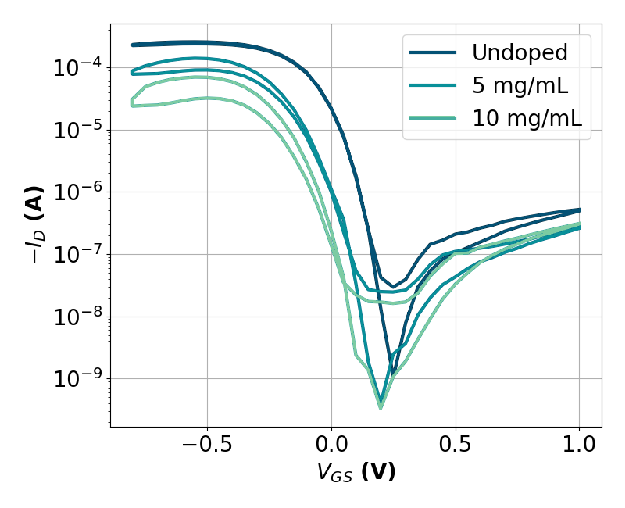
\includegraphics[width=5.5cm]{Images/pdf/Shift_Vds1.pdf} }}
    \subfloat[$V_{DS}$ = -0.3 V]{{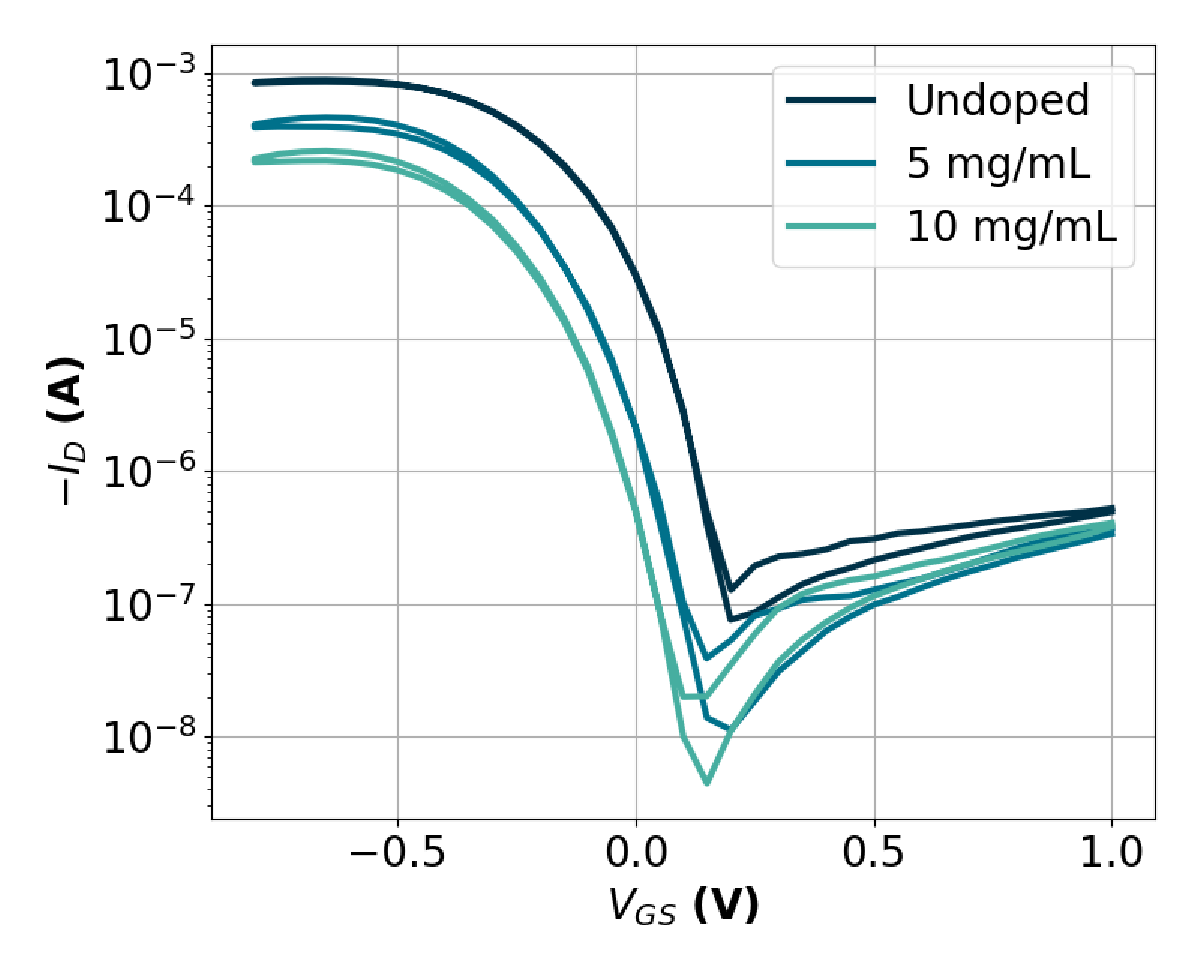
\includegraphics[width=5.5cm]{Images/pdf/Shift_Vds3.pdf} }}
    \qquad
    \subfloat[$V_{DS}$ = -0.5 V]{{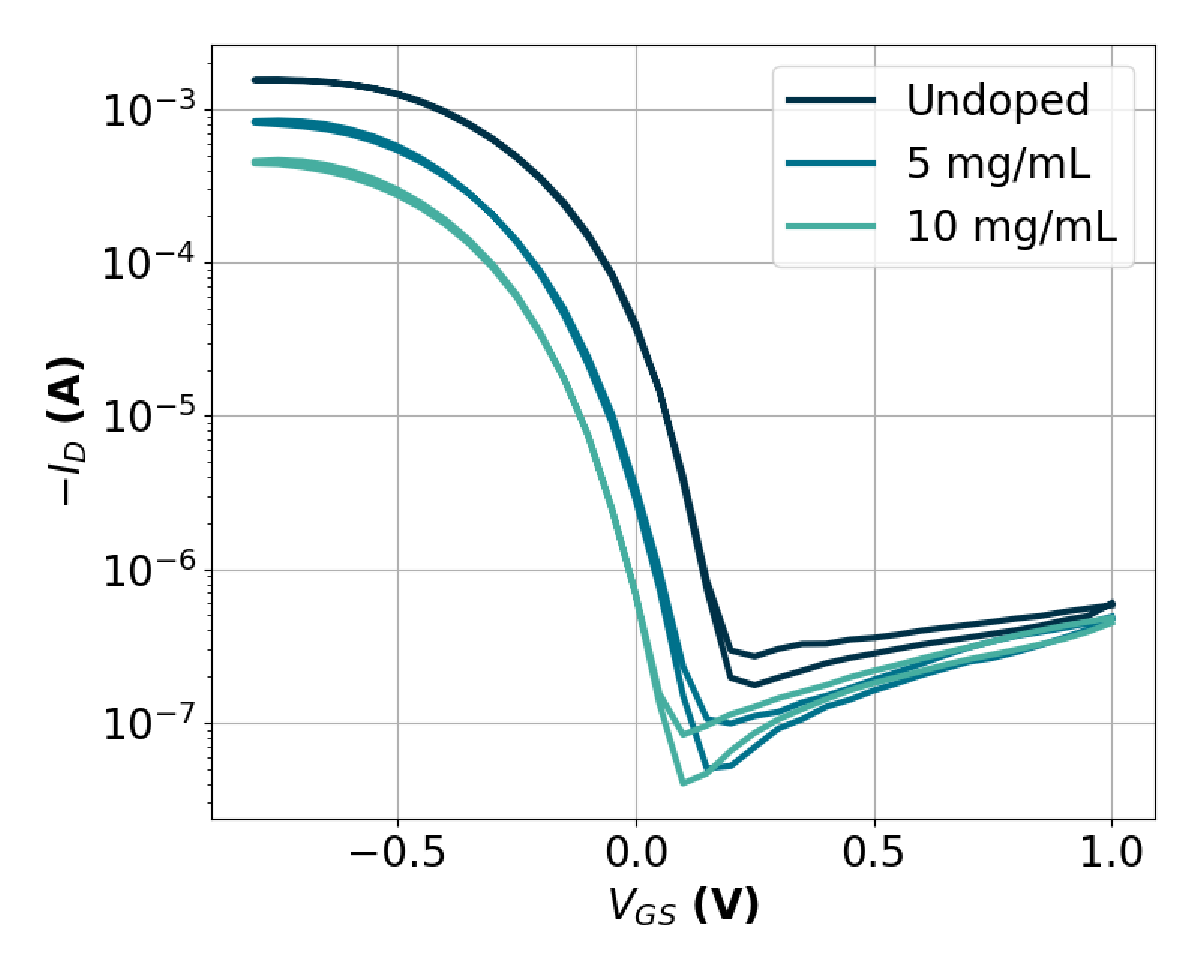
\includegraphics[width=5.5cm]{Images/pdf/Shift_Vds5.pdf} }}
    \subfloat[$V_{DS}$ = -0.7 V]{{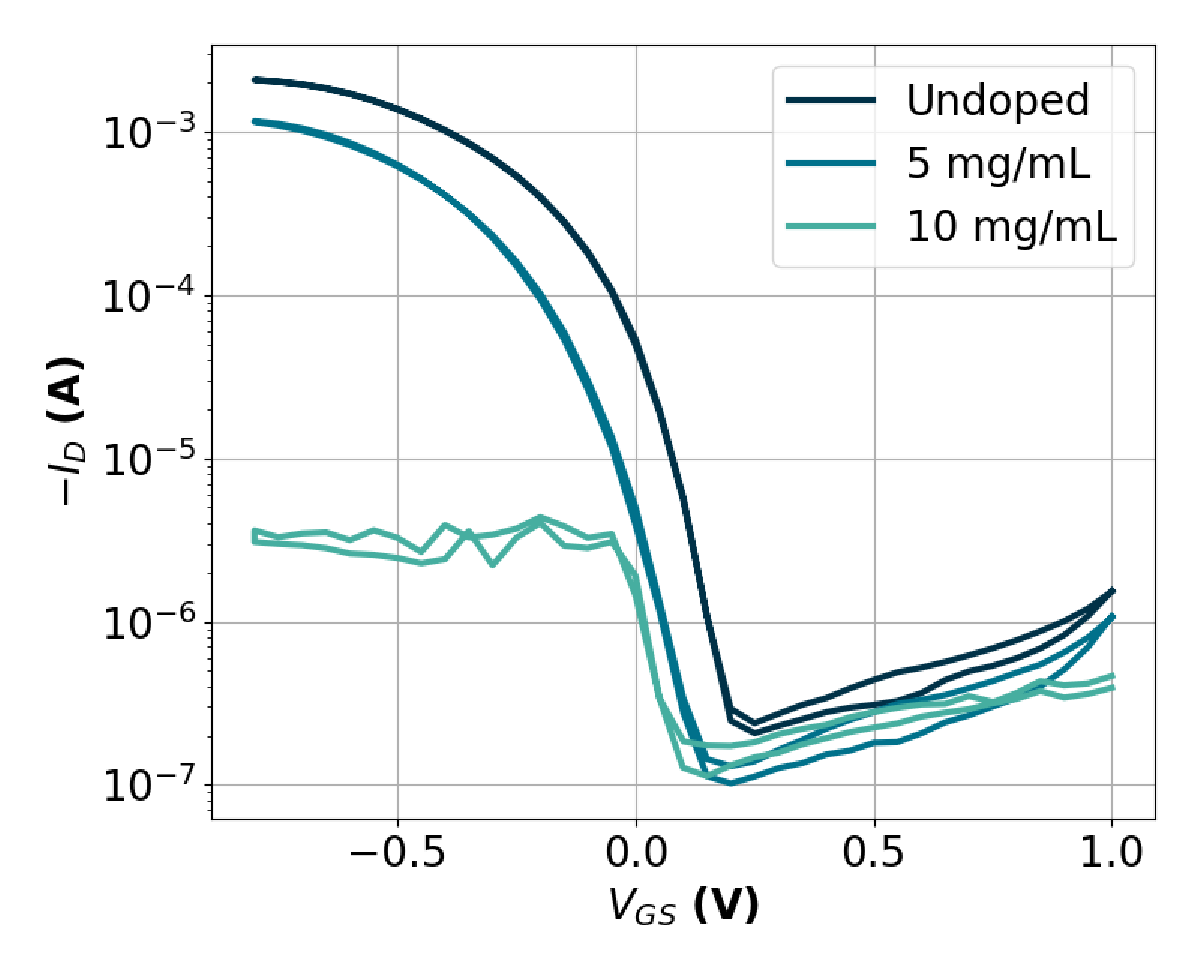
\includegraphics[width=5.5cm]{Images/pdf/Shift_Vds7.pdf} }}
    \caption[Transfer characteristics comparing different doping levels]{Transfer characteristics comparing undoped, 5 mg/mL and 10 mg/mL dopants devices, each graph represent a different $V_{DS}$}
    \label{fig:shift1}
\end{figure}

Additionally, threshold voltage values exhibited lower variability among different $V_{DS}$ values with higher doping levels, as despicted in Figure \ref{fig:vth_vds}. In the undoped device, the variability could be attributed to oxygen reduction reaction (ORR), which may differ under different drain bias conditions. In contrast, in the doped devices, this variability is expected to decrease since doping depletes reactive electrons from p(g3T2-T) with F$_{4}$TCNQ, ensuring better stability in air \cite{tanTuningOrganicElectrochemical2022}. %Further analysis needs to be done to confirm this hypothesis.  %Then although we are impacting mobility and repeatability among loops, the values at different drain biased are maintain. 

\begin{figure}[ht]
  \centering
  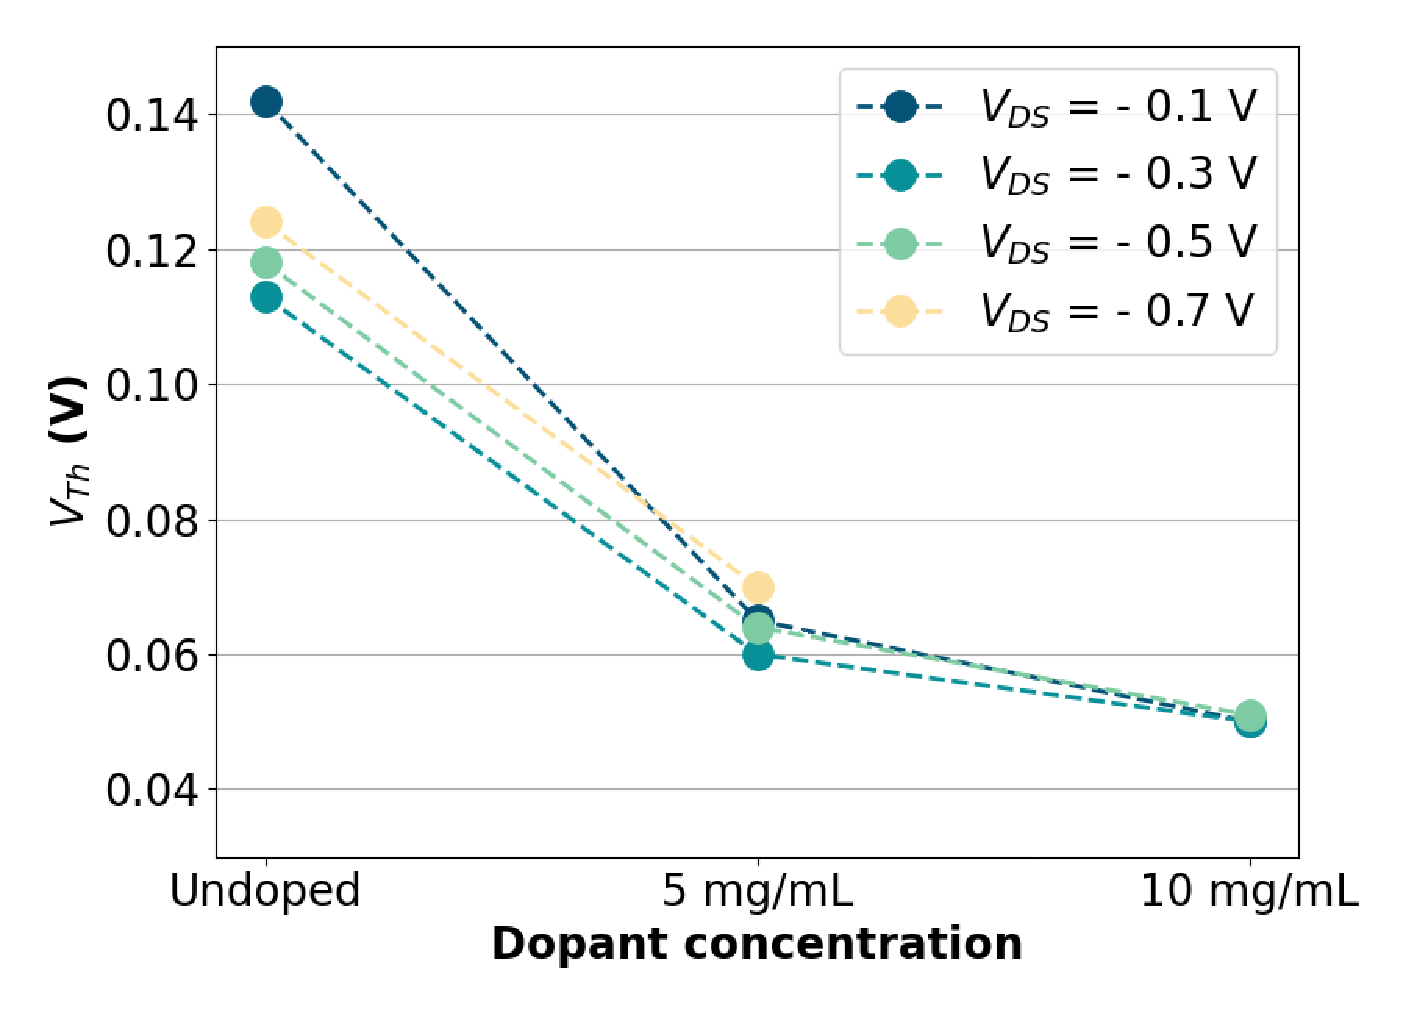
\includegraphics[width=8cm]{Images/pdf/vth_shift_vds.pdf}
  \caption[Threshold shift at different doping levels and $V_{DS}$]{Threshold shift at different doping levels and $V_{DS}$, calculations were done using data shown in Figure \ref{fig:transx2}.}
  \label{fig:vth_vds}
\end{figure}

Furthermore, while not presented in this report, it was observed during the analysis, that undoped OECT devices exhibit higher repeatability in transfer characteristics. The saturation of ORR in undoped species, as mentioned earlier, may contribute to this repeatability. However, the variability in doped species requires further study. %Potential for appendix
%but it is yet unclear. %An new hypothesis that could explained is to consider our environmental conditions as a infinite reservoir of molecular oxygen, until this unwanted doping and ORR reaches saturation, making it stable. In the case of F$_{4}$TCNQ, stability is still unclear and further investigation will be done in the next sections.

\subsection{Stability on Air of p(g3T2-T)}
The channel conductivity of an undoped device was measured immediately after spin-coating, yielding a value of 1 $\mu$S. After undergoing the patterning process described in the previous sections, the conductivity increased three orders of magnitude to approximately 1 mS. Even though, $\mu$S values already signify oxidation, the patterning process further oxidizes our material. %In this section, a way to revert this oxidation and find a compatible process to obtain accumulation-mode OECTs.
%Before getting into the revers

Measurements of $I_{D}$ at -0.3 V of $V_{DS}$ and no gate bias exhibited a small decrease of 4\% and small increase of 15\% within two hours in in $N_{2}$ and ambient air environments, respectively. This observation suggests that stability in ambient air is compromised due to unwanted doping.

A similar study was conducted with a doped device containing 5 mg/mL of F$_{6}TCNNQ$ dopant, resulting a higher level of doping compared to F$_{4}TCNQ$ at the same concentration, as detailed in Appendix A. The channel conductivity reached a value of 266 $\mu$S with a reduction of 1.2\% within one hour in $N_{2}$ environment and remained stable with minimal fluctuations of 1.0\% within one hour in ambient condition. This indicates a lower conductivity compared to the oxidized p(g3T2-T) but similar stability in air, as reported in reference \cite{tanTuningOrganicElectrochemical2022}.

Remarkably, upon contact with SSE precursor, conductivity of both samples drops significantly, approximately six orders of magnitude, in a $N_{2}$ environment, reaching the sensitivity limits of our equipment and resulting in a noisy signal, as shown in Figure \ref{fig:revox1}A. One plausible explanation is that p(g3T2-T), as a type VI OMIEC, lacks chemical binding with $TCNQ^{-}$ anions. When in contact with the electrolyte, the anions are drawn away from the polymer backbone (de-doping), restoring its original insulating state, which is essential for accumulation-mode OECTs.
%\begin{table}[ht]
%\centering
%\caption{Conductivity measurements of undoped p(g3T2-T)}
%\begin{tabular}{l|c}
%Condition  & Conductivity (S) \\\hline
%Unpatterned & 1.3 $\times$ 10^{-6} \\
%Patterned & 1.0 $\times$ 10^{-3} \\
%\end{tabular}
%\label{tab:cond}
%\end{table}

\begin{figure}[ht]
    \centering
    \subfloat[]{{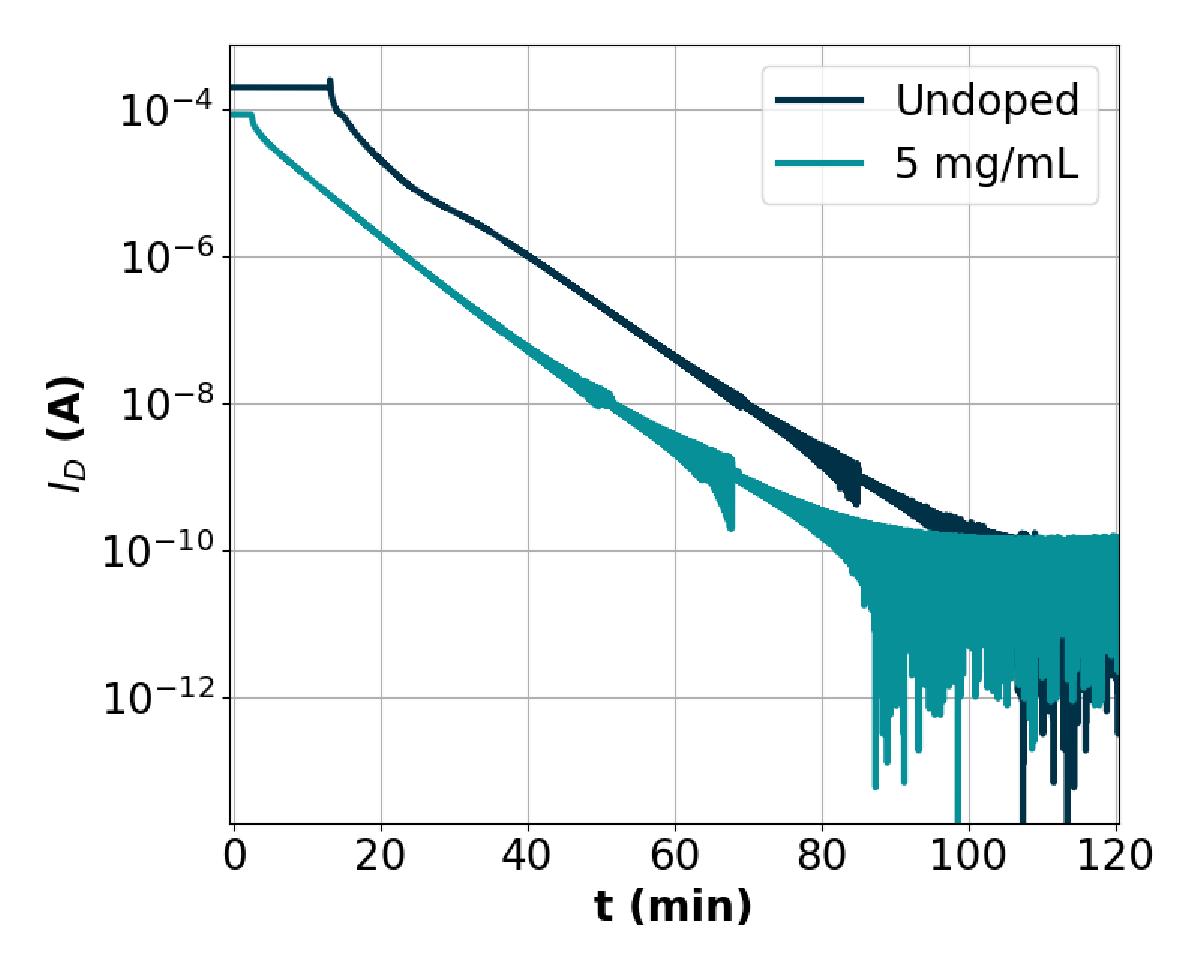
\includegraphics[width=6.5cm]{Images/pdf/revox_gb_only.pdf} }}
    %\qquad
    \subfloat[]{{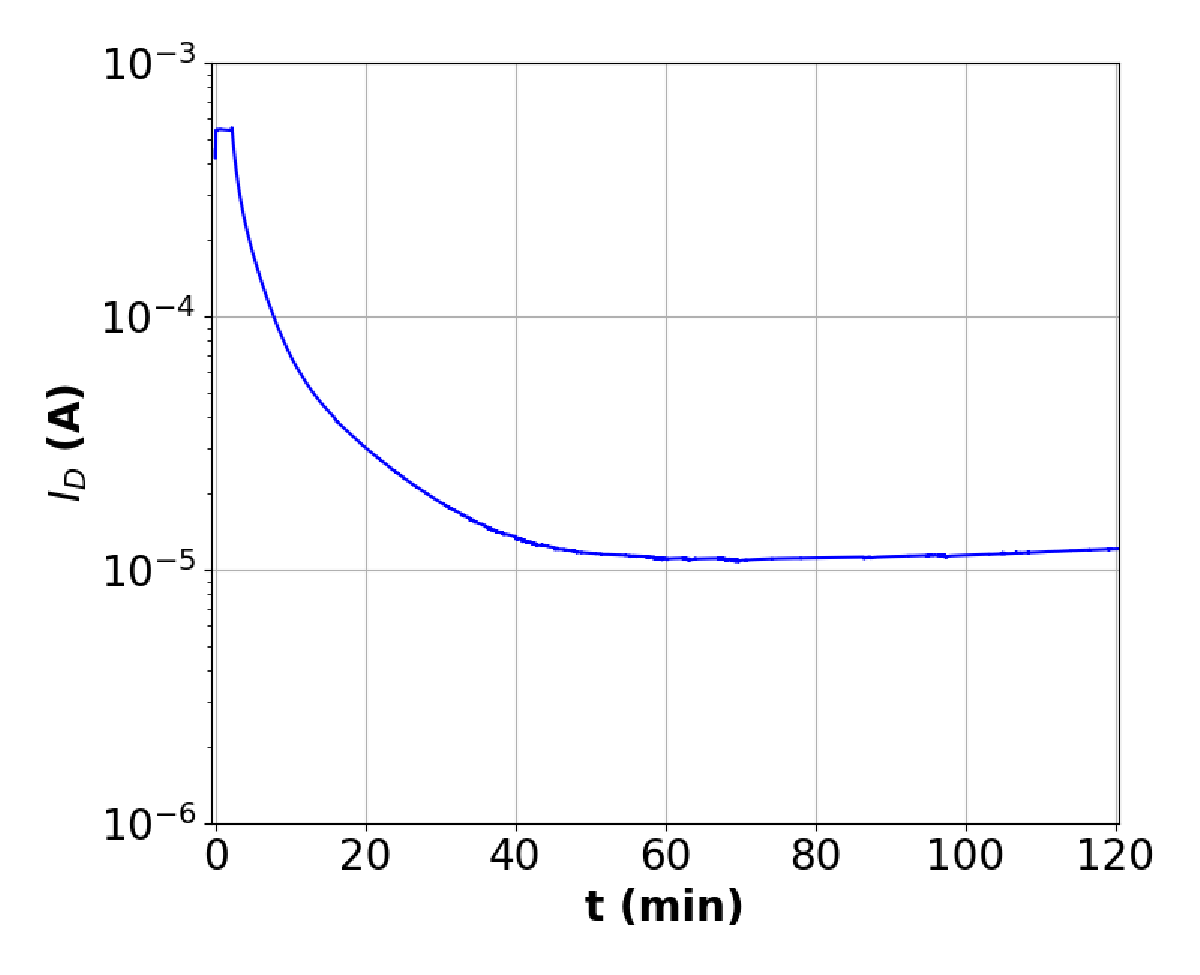
\includegraphics[width=6.5cm]{Images/pdf/revox_air.pdf} }}
    %\subfloat[Ambient and $N_{2}$ environment]{{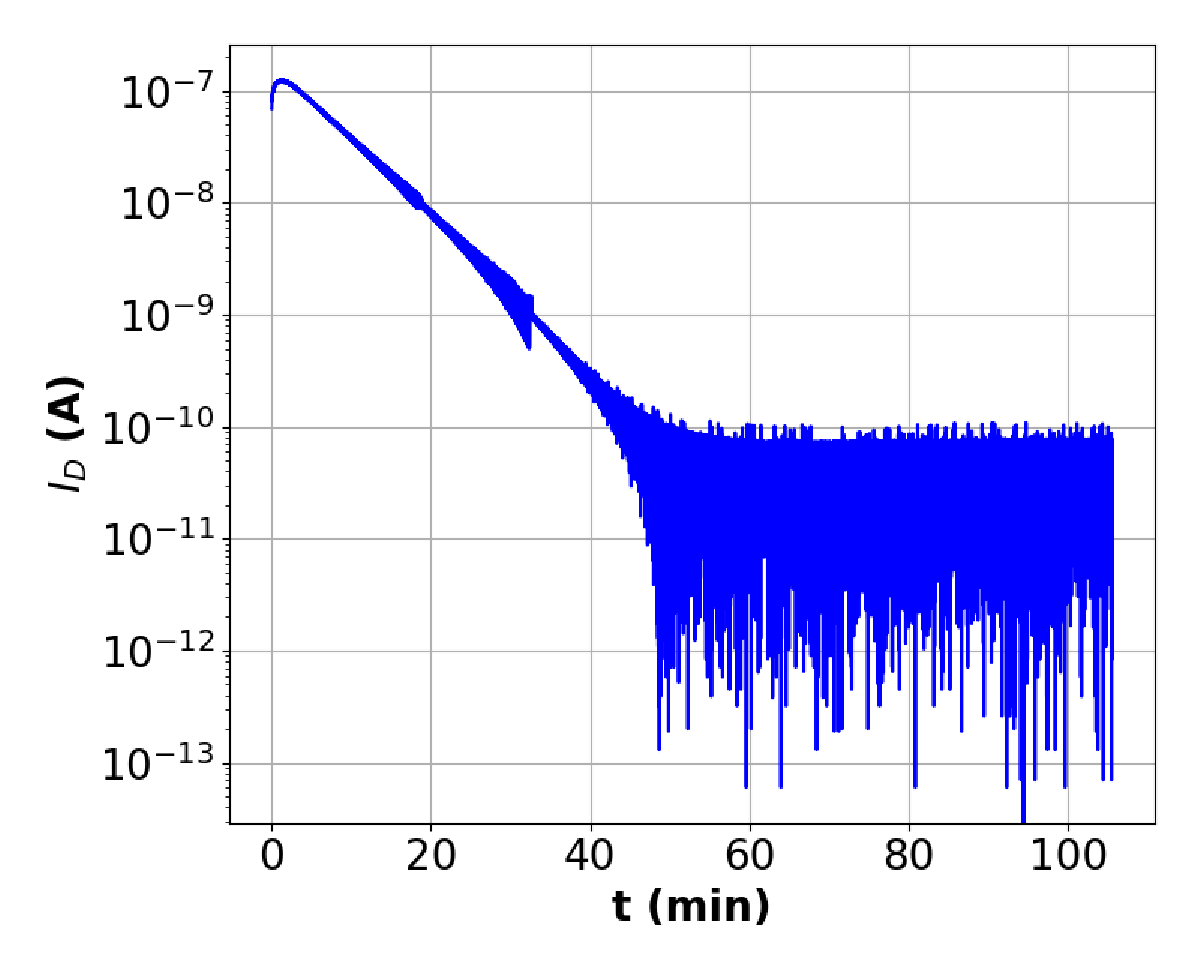
\includegraphics[height=5.5cm]{Images/pdf/revox_gb_afterair.pdf} }}
    \caption[Drain current over time of undoped-p(g3T2-T) coupled with SSE precursor]{Drain current over time of undoped p(g3T2-T) coupled with SSE precursor under A) $N_{2}$, and B) ambient environment%, C)$N_{2}$ environment after B)
    .}
    \label{fig:revox1}
\end{figure}

Under ambient conditions, there is a smaller decrease of slightly more than one order of magnitude for the undoped sample, as seen in Figure \ref{fig:revox1}B. The doped sample initially exhibited a similar but faster drop within the first 15 minutes, followed by a sudden increase of $I_{D}$. In both scenarios, the ORR prevented a greater decrease in current. The fluctuation seen in the doped species may be attributed to the simultaneous occurrence of irreversible de-doping $TCNQ^{-}$ anions and ORR . %Another undoped sample share the same results.

\begin{figure}[ht]
    \centering
    %\subfloat[N$_{2}$ environment]{{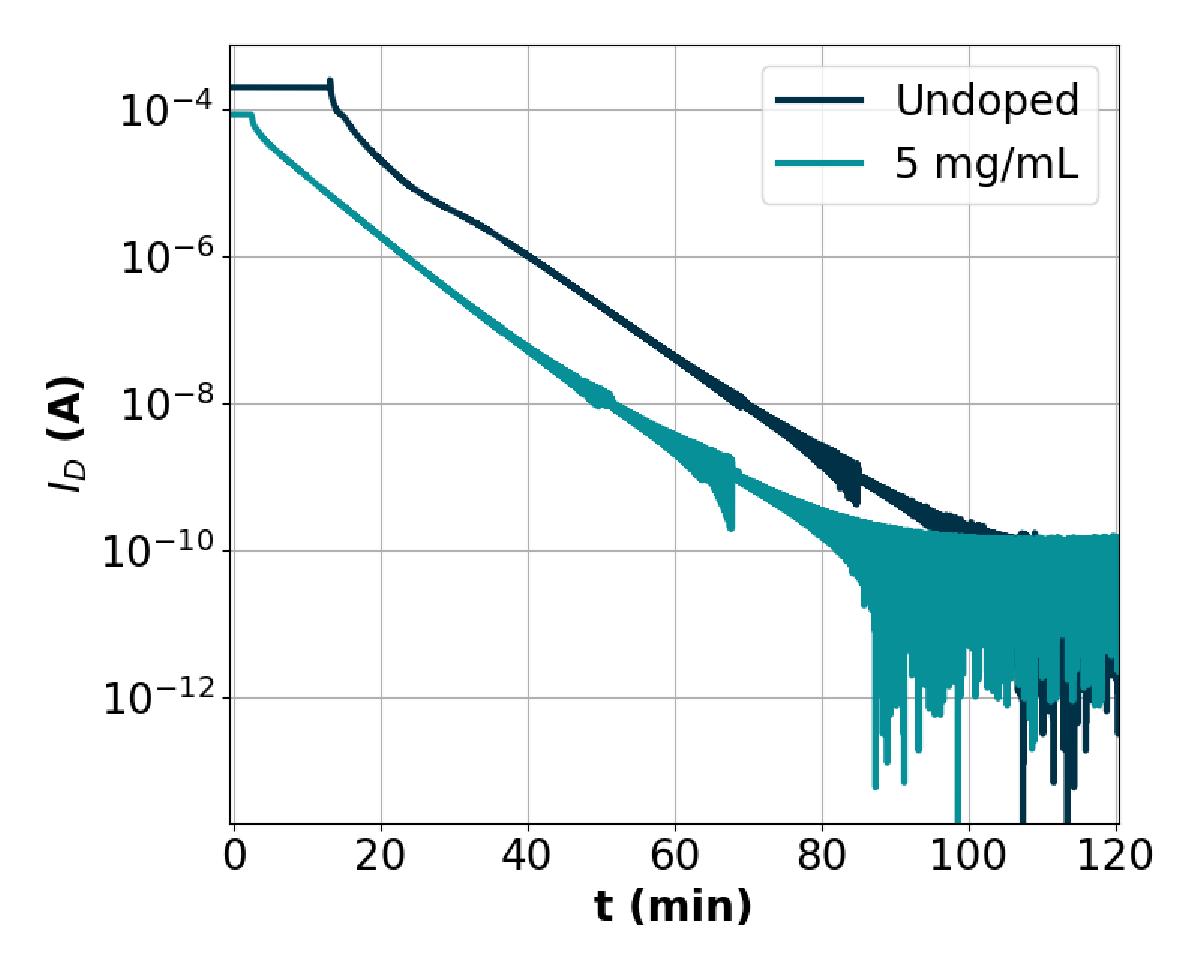
\includegraphics[width=5.5cm]{Images/pdf/revox_gb_only.pdf} }}
    %\subfloat[Transfer in ambient]{{
    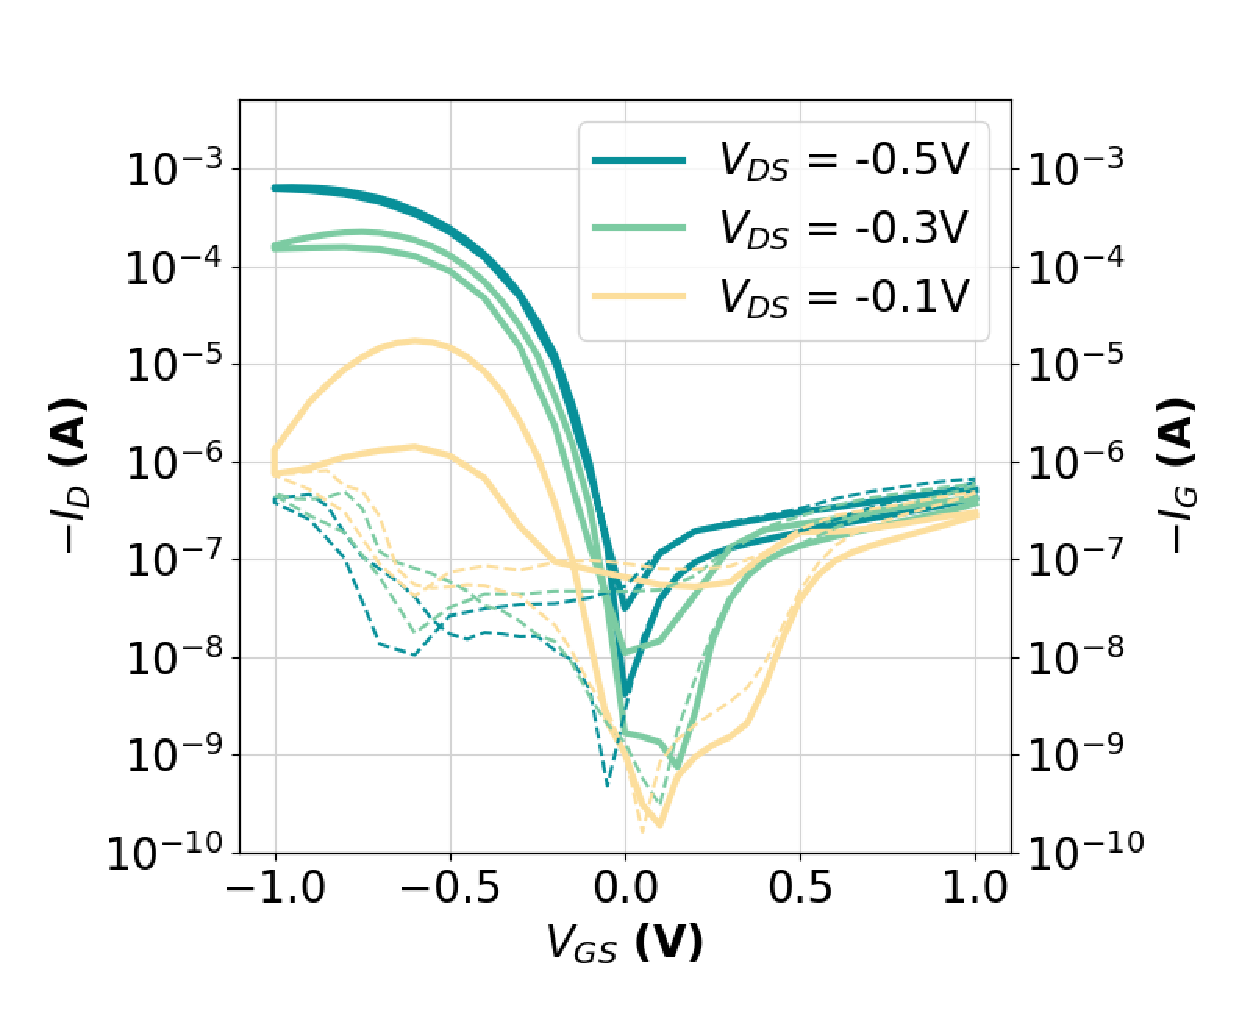
\includegraphics[width=6.5cm]{Images/pdf/revox_transfer_loop2.pdf}% }}
    \caption[Transfer characteristics after electrochemical de-doping]{Transfer characteristics after electrochemical de-doping at different $V_{DS}$ under ambient conditions}
    \label{fig:transrevox1}
\end{figure}

Transfer curves of the undoped device using an Ag/AgCl pellet as gate, were measured under ambient conditions after de-doping in $N_{2}$ environment, as despicted in Figure \ref{fig:transrevox1}. The device exhibited shifts in its ON voltage and negative threshold voltages values, as summarized in Table \ref{tab:vth_air}, moving towards negative values. A visible sign of degradation was perceived at the end of the measurements when $V_{DS}$ is -0.1 V.

\begin{table}[ht]
\centering
\caption{Threshold voltage extracted from Figure \ref{fig:transrevox1}}
\begin{tabular}{c|c}
 $V_{DS}$ [V] & $V_{Th}$ [V] \\\hline
-0.1 & -0.18 \\
-0.3 & -0.15 \\
-0.5 & -0.13 \\ \hline
\end{tabular}
\label{tab:vth_air}
\end{table}

In summary, a pre de-doping step could potentially serve as a method for obtaining accumulation-mode OECTs by reversing the oxidation of p(g3T2-T), and will be explored in the following section.

\subsection{Reverse Oxidation of Undoped-p(g3T2-T)}
Based on previous the analysis, it took approximately two hours to fully de-dope p(g3T2-T) and reach an insulating state of the polymer. However, this process could be expedited by applying a positive gate bias to one of the devices.

Additionally, the use of high-temperature baking step to revert the oxidation of an p(g3T2-T) OECT %was a method suggested by colleagues in the Biosens group at IAPP and 
will also be tested.   

\subsubsection{By Electrochemical Dedoping}
De-doping in a $N_{2}$ environment was performed by applying a +1 V gate bias. p(g3T2-T) reached its insulating state in less than 300 seconds, significantly faster than observed in the previos section. However, it was expected that this process would not be reversible upon disconnection of the gate. Figure \ref{fig:revox2}A confirms this expectation: after $I_{D}$ drastically dropped and the gate was disconnected (gray arrows), the current remained low, and leakage current is predominant. When the gate was reconnected (gold arrows), a capacitive current spike occurred but later stabilized to match the leakage current.

\begin{figure}[ht]
    \centering
    \subfloat[]{{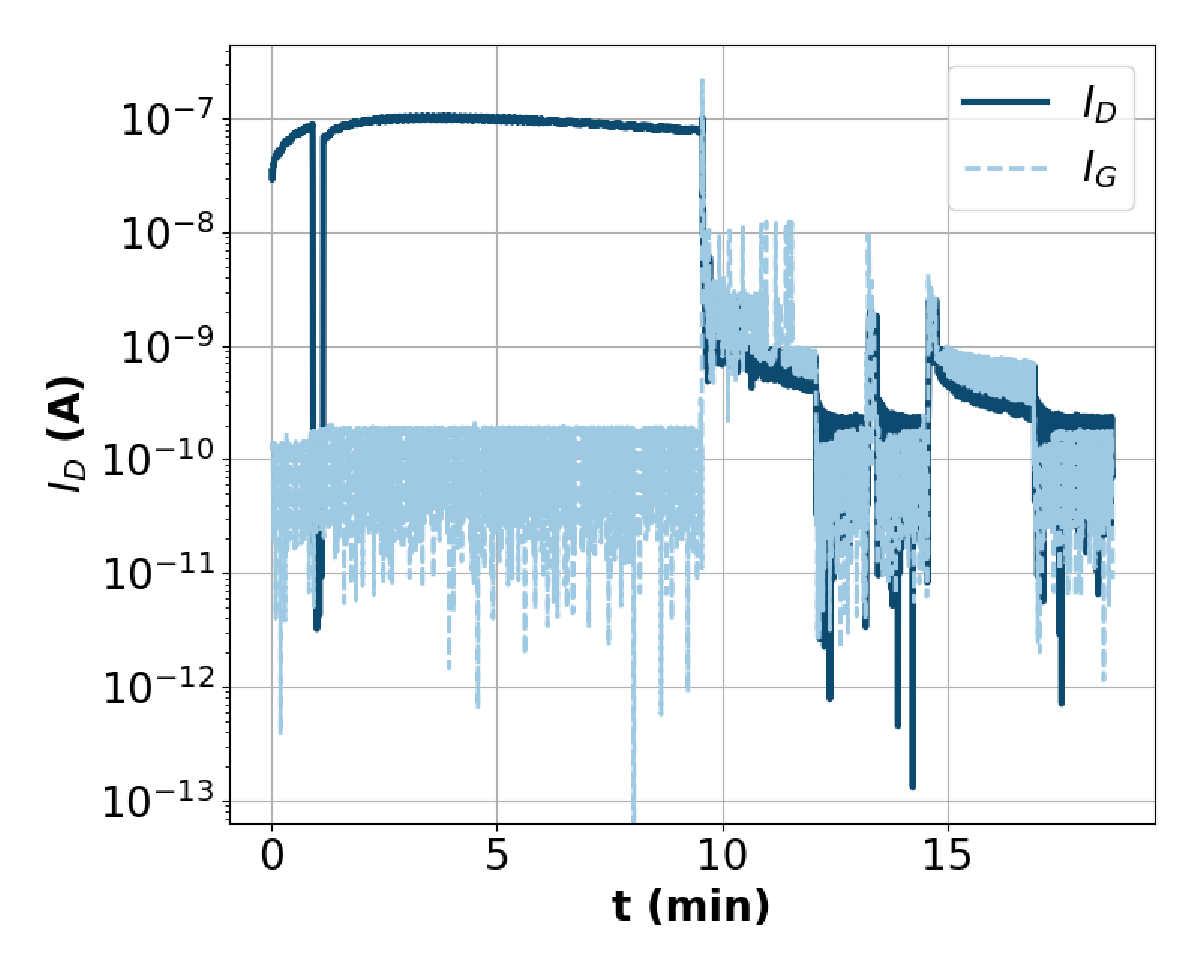
\includegraphics[width=6cm]{Images/pdf/elec-dedop1.pdf} }}
    \subfloat[]{{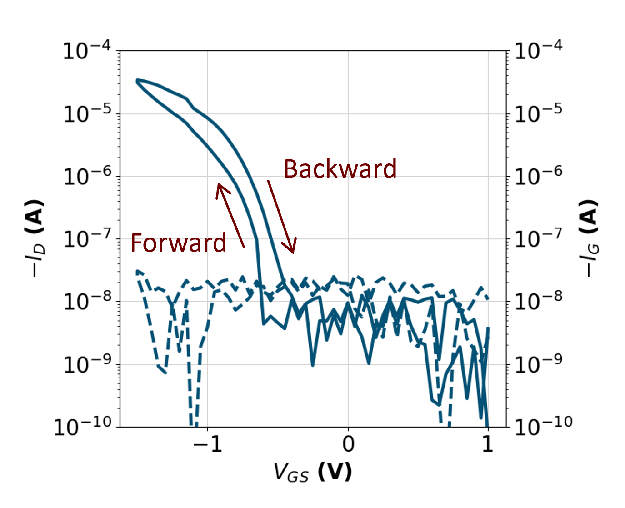
\includegraphics[width=6.5cm]{Images/pdf/transfer_de-dop.pdf}}}
    \caption[Electrochemical de-doping of oxidized p(g3T2-T) OECT]{A) De-doping p(g3T2-T) using a gate biased of +1V, gold arrows indicate gate connection, while grey arrows indicate when gate was disconnected. B) Transfer characteristic at $V_{DS}$ of -0.1 V using p(g3T2-T) gate coupled with SSE precursor.}
    \label{fig:revox2}
\end{figure}

Transfer curves using the p(g3T2-T) gate showed a negative turn-on voltage after reversing oxidation (Figure \ref{fig:revox2}B). However, it was perceived that using the OMIEC gate instead of the Ag/AgCl pellet affects our ``gating efficiency'', as expected. Weissbach et al.  \cite{weissbachUnravelingElectrochemicalElectrode2023} demonstrated the Electrochemical Electrode Coupling (ECC) between channel and its electrode has a more pronounce effect on device operation when micro-integrated polarizable gates (OMIECs) are used. This can result in saturation loss (as seen in Figure \ref{fig:revox2}B) and threshold voltage roll-of when increasing $V_{DS}$. This was observed during measurements. Therefore, moving forward, $V_{DS}$ will be fixed at -0.1 V.

\subsubsection{By Heating}


\subsection{Solid-OECTs using Undoped-p(g3T2-T)}
The fabrication of OECTs using a solid-state electrolyte at IAPP, to enable IC and thermodynamics studies, was established in reference  \cite{weissbachPhotopatternableSolidElectrolyte2022}. The SSE consists of monomer units, including NIPAm and HHPA, as outlined in Section \ref{tab:sse} in Chapter \ref{cha:2}. %such as N-isopropylacrylamide (NIPAm) and 2-hydroxy4’-(2-hydroxyethoxy)-2-methylpropiophenone (HHPAA) 
Upon exposure to UV light, these monomers cross-link, forming the polymer poly(N-isopropylacrylamide) (PNIPAm), which is more precisely considered as a rigid gel. 

Two types of OECTs were tested under a $N_{2}$ environment and later exposed to ambient conditions. In one type, SSE couples all fourteen devices in the sample, while in the other type, each device possesses a microstructure SSE. The latter strategy enhances the performance of OECTs by minimizing leakage current and avoiding device crosstalk. This can be achieved through a photolithography process, as outlined in reference \cite{weissbachPhotopatternableSolidElectrolyte2022}, or by inkjet printing, as implemented by team members. Both methods were employed under normal cleanroom conditions to determine which  approach minimizes oxidation or allows for the reverse oxidation of p(g3T2-T) within the process. 

In this subsection, a total of three samples will be analyzed, it is expected to have low degree of oxidation in all devices.

%Finally, one of each type of sample was exposed to air to understand ORR effects. It is expected to see oxidation in all devices.

\subsubsection{OECT with Drop-casted SSE}%Solid-State Electrolyte}
At this point, the patterning process had improved its yield, with twelve out of the fourteen devices being successfully patterned, although there were some variations in thickness, as evidenced by the reflection hue of the micrographs. Among these devices, only seven remained operational. A representative device can be seen in Figure \ref{fig:dropcast}A.  %among them, one with high conductivity and six with low conductivity that exhibited transfer characteristics similar to Figure \ref{fig:revox2}B. 
 %by improving homogeneity of dynamic spin-coating, say patterning number, 

\begin{figure}[ht]
    \centering
    \subfloat[]{{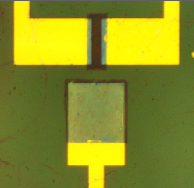
\includegraphics[width=3cm]{Images/pdf/und_device.pdf} }}
	\hspace{3em}    
    \subfloat[]{{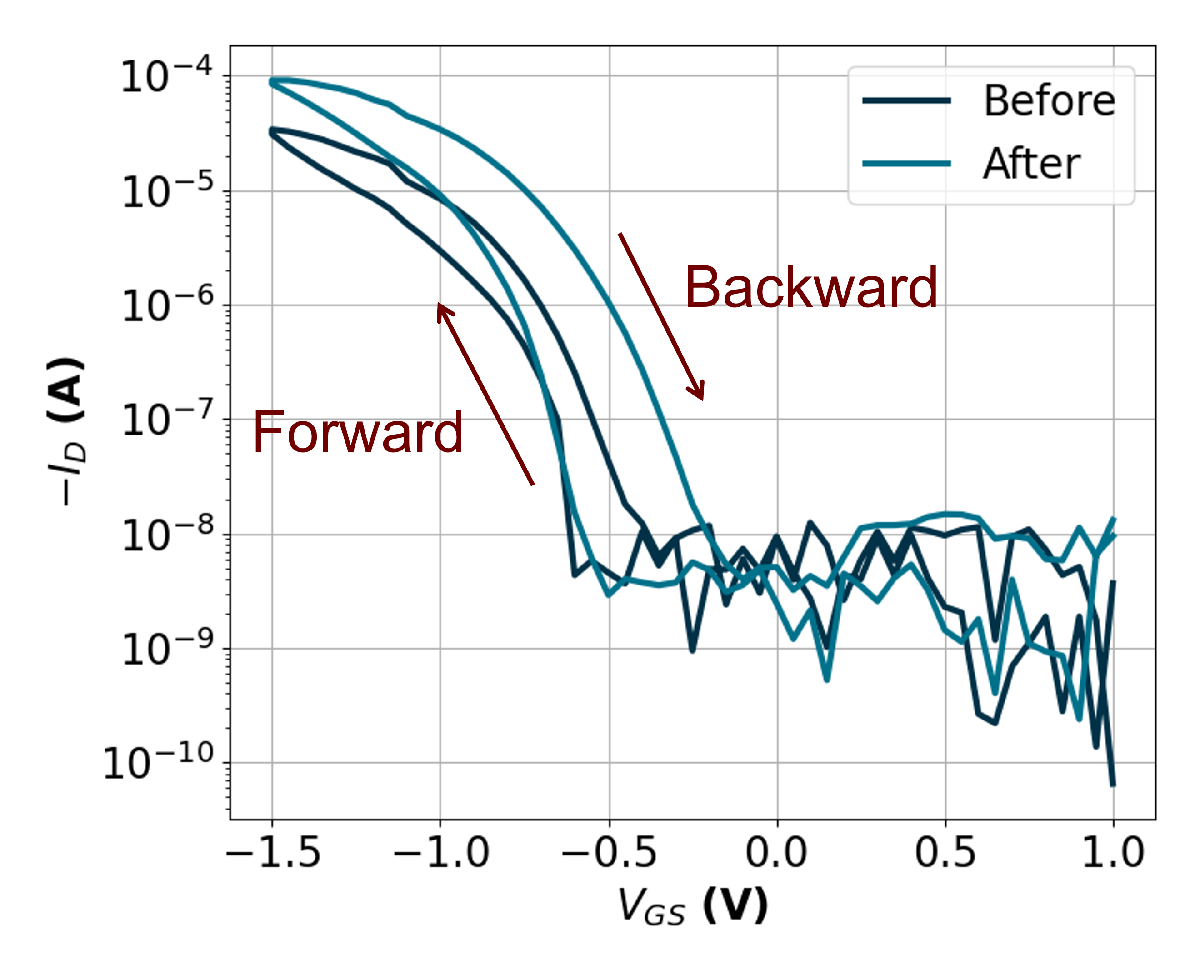
\includegraphics[width=6cm]{Images/pdf/transfer_de-dop_exp.pdf} }}
    \qquad
    \subfloat[]{{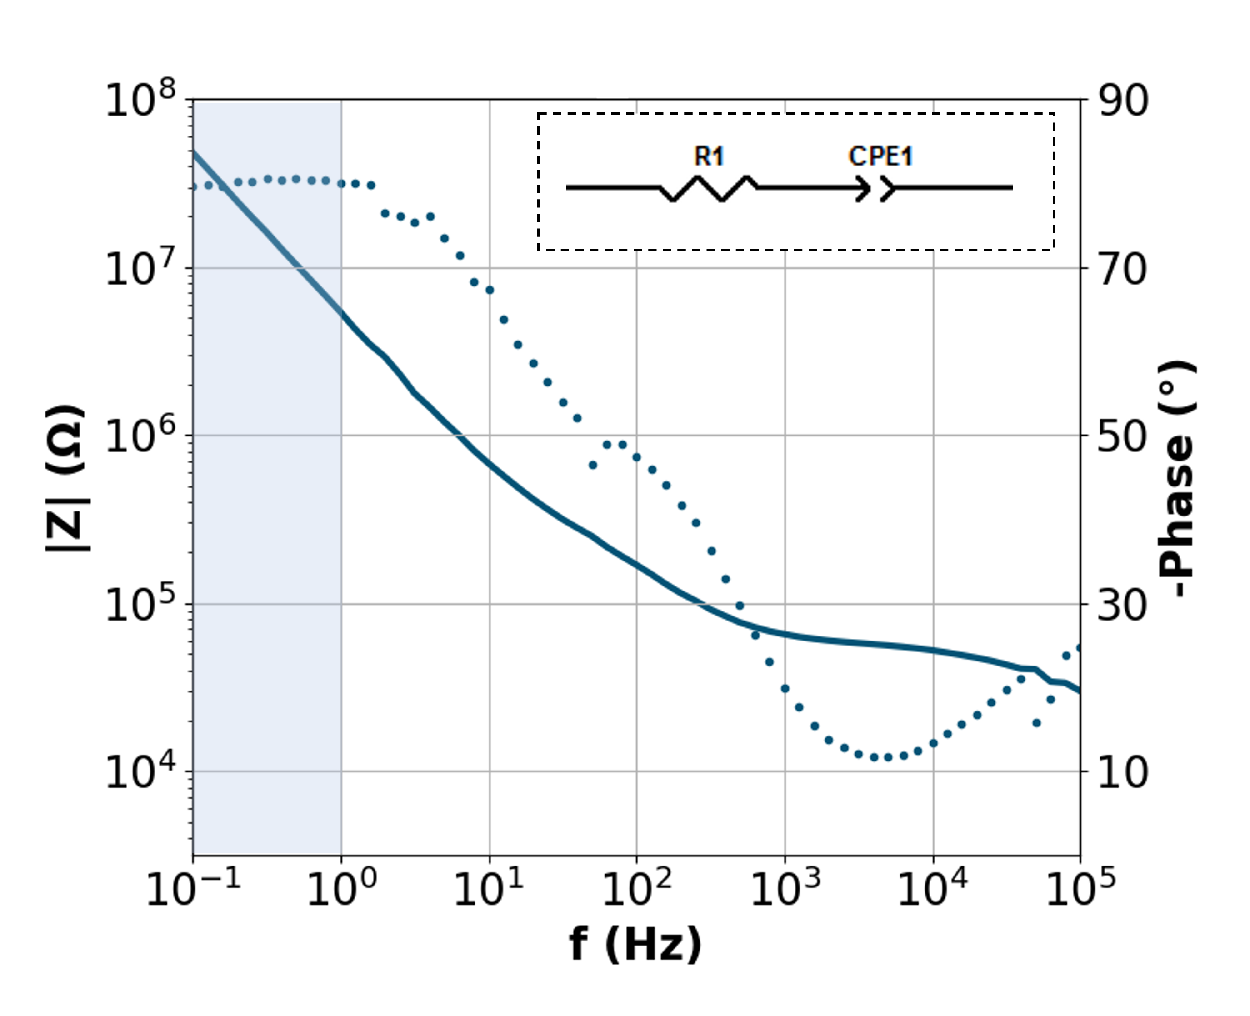
\includegraphics[width=6cm]{Images/pdf/EIS_drop.pdf} }}
    \subfloat[]{{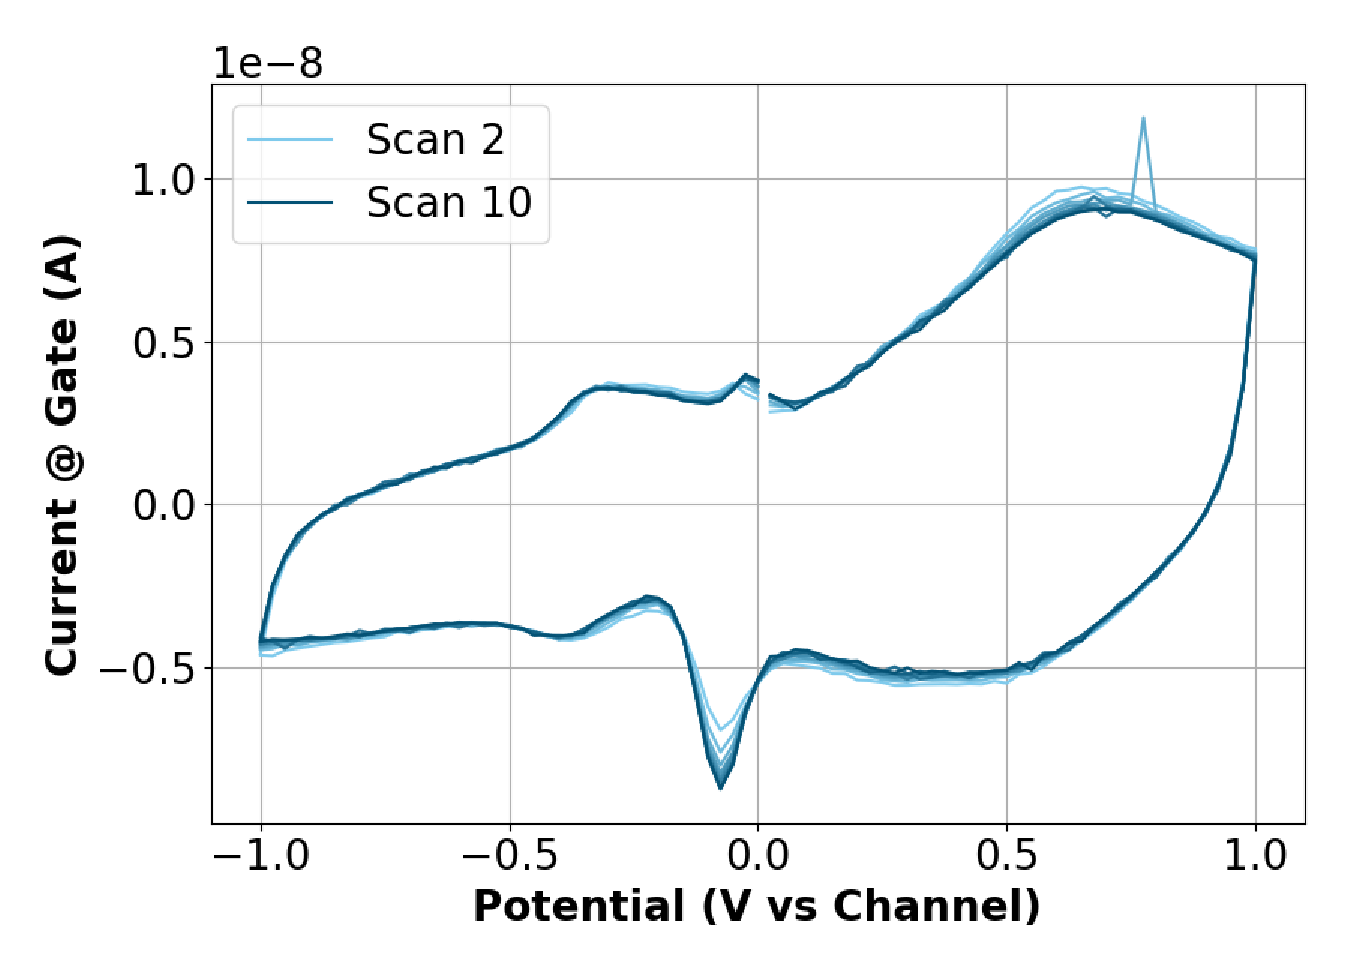
\includegraphics[width=6cm]{Images/pdf/CV_drop.pdf} }}
    \caption[Performance of solid-OECT with drop-casted SSE]{A) Micrograph of patterned device before application of SSE, B) transfer characteristics before and after exposure at $V_{DS}$ of -0.1 V. And representative C) Bode plot obtained by EIS and C) redox behavior between Au/p(g3T2-T) and SSE using CV.}
    \label{fig:dropcast}
\end{figure}

Electrochemical de-doping of one device in the sample was carried out before exposure. Measurements of channel conductivity of the other devices indicated an impact of this process to neighbouring devices (a total of 5) as most of them had very low conductivity, in the order of nS. One exception exhibited a conductivity in the order of the $\mu$S and a threshold voltage of 0.0 V. Moreover, attempts to perform irreversible electrochemical de-doping on this device after exposure (cross-linking of monomer units) were unsuccessful. It appeared that the formation of PNIPAm prevented irreversible de-doping. This outcome is crucial for the fabrication of doped-devices and will be discussed further in Section \ref{dopedOECTs}.

Transfer characteristics were measured both before and after exposure, as seen in Figure \ref{fig:dropcast}B. An increase in current upon crosslinking is observed, and threshold voltages were calculated for forward and backward scans, the values are presented in Table \ref{tab:dropfom}. A small hysteresis was perceived but further analysis was considered beyond the scope of this work. Importantly, negative threshold voltages were calculated in all devices with low conductivity.

The shadowed area of the Bode plot illustrated in Figure \ref{fig:dropcast}C (low frequencies) was used to calculate the channel capacitance and volumetric capacitance, as shown in Table \ref{tab:dropfom}. Very low values were obtained, which may indicate ongoing oxidation or the presence of defects (i.e. remnants of photoresist). %Additionally, the geometry of the devices could contribute to these low capacitance values

Furthermore, redox potentials were extracted from cyclic voltammetry measuerements, as shown in Figure \ref{fig:dropcast}D. The oxidation peak and two reduction peaks are listed in Table \ref{tab:dropfom}. 

It is important to clarify that the redox peaks extracted from these measurements do not exclusively represent reduction and oxidation potentials between the working electrode (Au/p(g3T2-T)) and electrolyte. This is because the counter electrode and reference electrode are shorted and connected to the channel, which should be significantly large to minimize its effects on the electrolyte. Instead, these peaks represent crucial operation points for our OECT, where electron transfer is more pronounced. 

For instance, the oxidation peak may signify both the oxidation and the reduction of the channel, and the same applies to the reduction peaks. Furthermore, particularly for these case, peaks occurring away from the vicinity of 0 V could indicate interaction with oxygen or the presence of defects in our devices.

%%D7
\begin{table}[ht]
\centering
\caption{Parameters extracted from the characterization of drop-casted SSE OECT}
\begin{tabular}{l|c||l|c}
Parameters & Value & Parameters & Value \\\hline \hline
V$_{Th,forward}$ [V] & -0.21 $\pm$ 0.13 & V$_{Th,backward}$ [V] & -0.17 $\pm$ 0.08\\
& & &\\[-1em]
C$_{channel}$ [nF] & 27.6 & C* [Fcm$^{-3}$] & 29.7 \\
%C$_{channel}$ [nF] & 36 $\pm$ 10 & C* [Fcm$^{-3}$] & 38 $\pm$ 10 \\
& & &\\[-1em]
V$_{ox}$ [V] & 0.68 $\pm$ 0.02 & V$_{red}$ [V] & -1.0, -0.1 \\
& & &\\[-1em]
|g$_{m,max}$| [mS] &  &  &\\\hline
\end{tabular}
\label{tab:dropfom}
\end{table}

Upon exposure to ambient conditions, a negative threshold voltage was maintained (-0.14 V with Ag/AgCl pellet), suggesting that drop-casted SSE creates a protective barrier against molecular oxygen.%, but still some interactions due to the redox peaks. (may need measurements outside for this one)

\subsubsection{OECT with Photopatterned SSE} %Solid-State Electrolyte}
This trial resulted in ten out of fourteen operational devices. A micrograph of a representative device can be seen in Figure \ref{fig:photoSSE}A. However, some devices exhibited unusual behavior due to defects and SSE partially blew off the device, and were excluded from the analysis.

The microstructure SSE on top of the device required the use of an adhesion promoter, unlike drop-casted SSE. In this particular case, where the removal of non-crosslinked SSE precursor was achieved using a $N_{2}$ gun, the risk of blowing off crosslinked SSE was not as high with the use of an adhesion promoter. Furthermore, the ethanol rinsing and high-temperature baking helped to counteract the oxidation of the polymer. The former led to the reaction described below: \\

%C_{2}H_{6}O_{(l, ethanol)} + 2O_{2}_{(g)} \arrow 2 CO_{2}_{(g)} + 3H_{2}O_{(g)}
\ce{\centering C2H6O_(l) + 2O2_(g) -> 2CO2_(g) + 3H2O_(l)} 
\\

The micrograph in Figure \ref{fig:photoSSE}A represents a patterned device before the application of the adhesion promoter, and signs of oxidation are evident by the brownish hue. 

After the application of SSE precursor and exposure, the transfer curves (seen in Figure \ref{fig:photoSSE}B) indicate slight hysteresis, turn-on voltages close to zero, and slightly negative threshold voltages, as shown in Table \ref{tab:photofom}. These values are higher compared to the samples with drop-casted SSE. 

\begin{figure}[ht]
    \centering
    \subfloat[]{{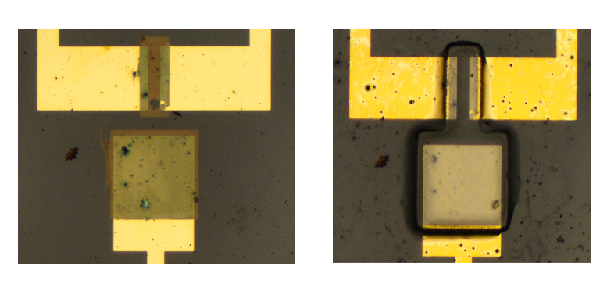
\includegraphics[width=6cm]{Images/pdf/und_photo.pdf} }}
    \hspace{2em}
    \subfloat[]{{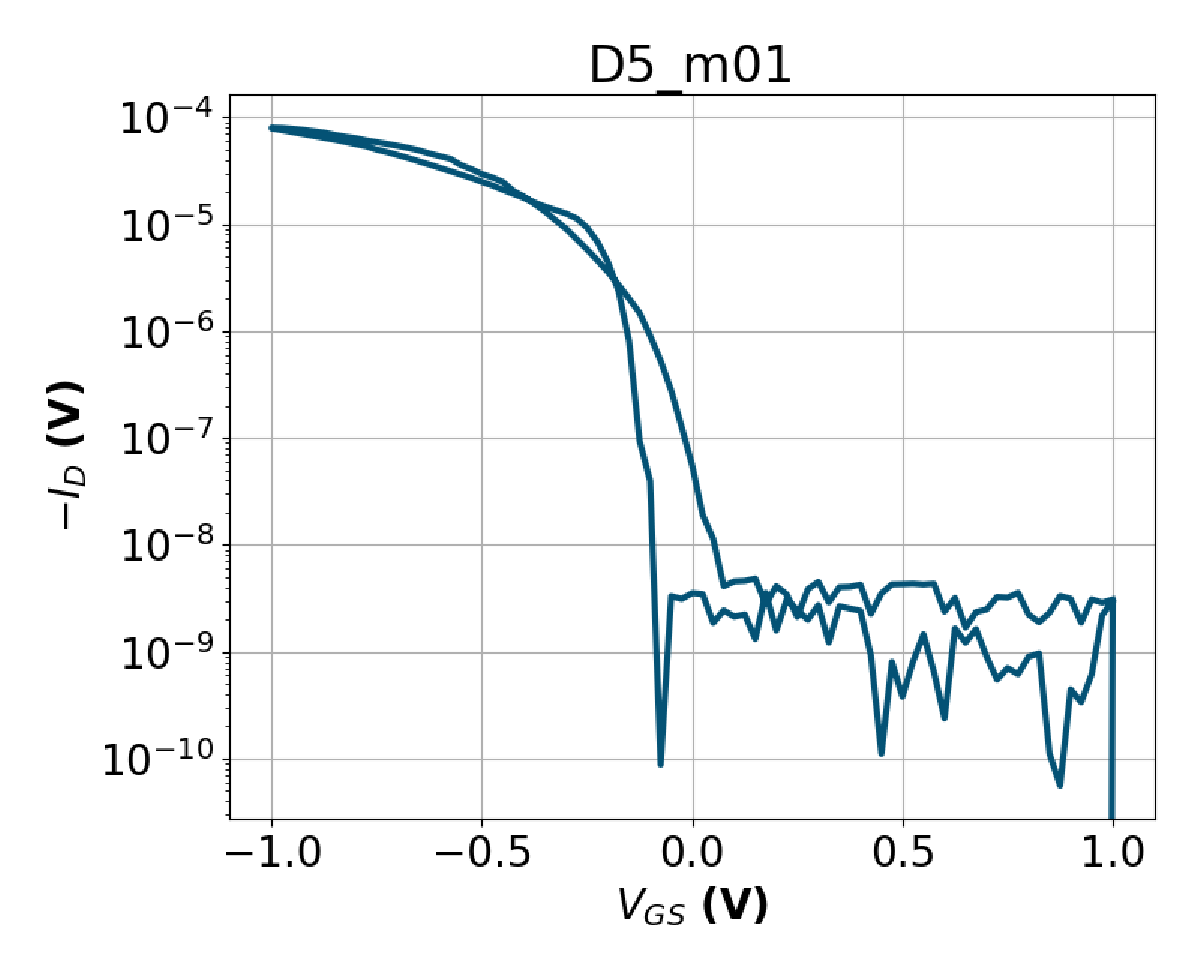
\includegraphics[width=6cm]{Images/pdf/transfer_photo.pdf} }}
    \qquad
    \subfloat[]{{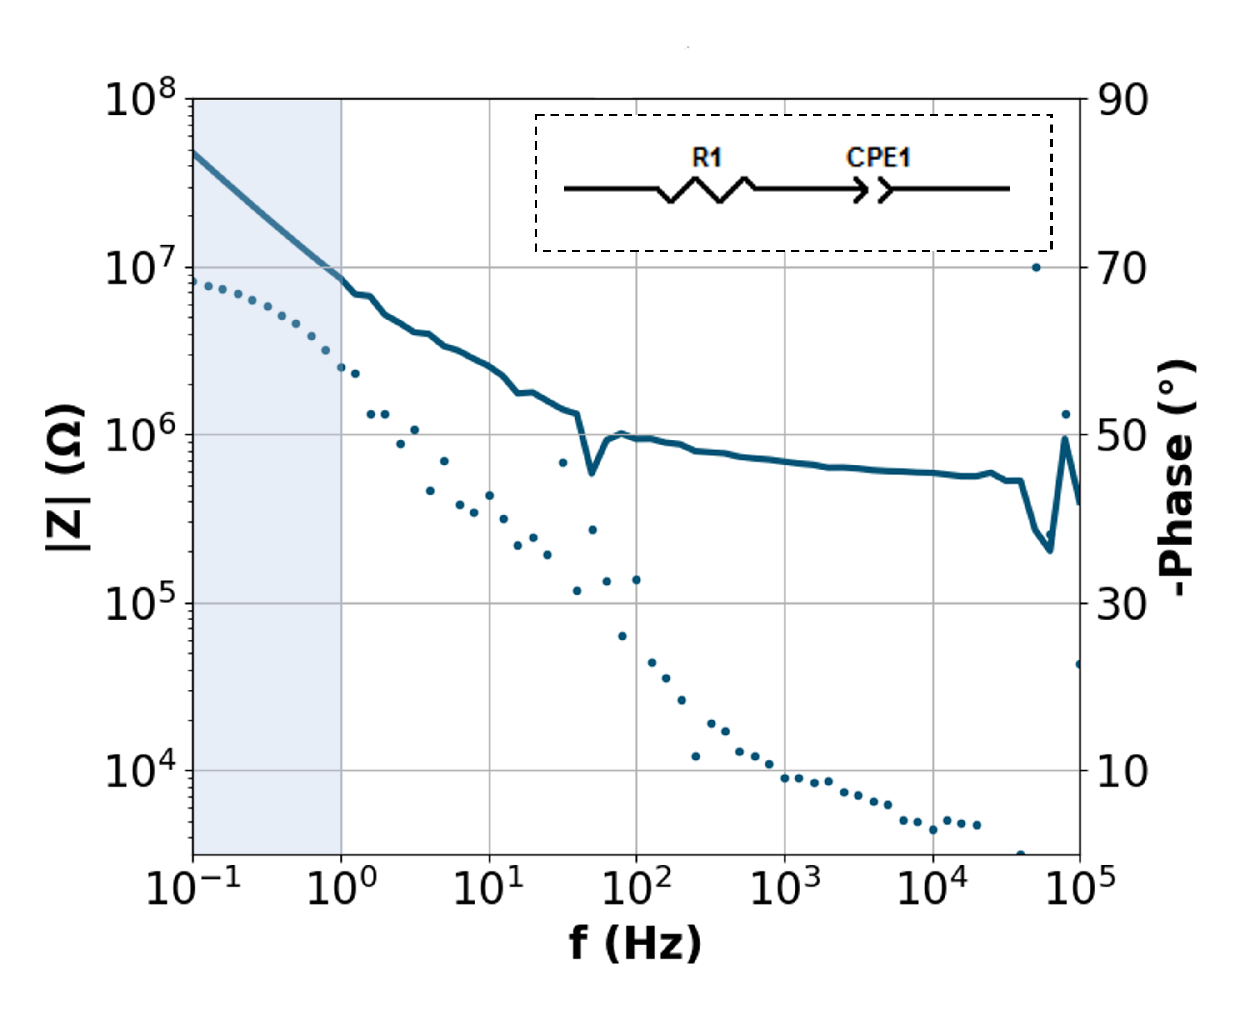
\includegraphics[width=6cm]{Images/pdf/EIS_photo.pdf} }}
    \subfloat[]{{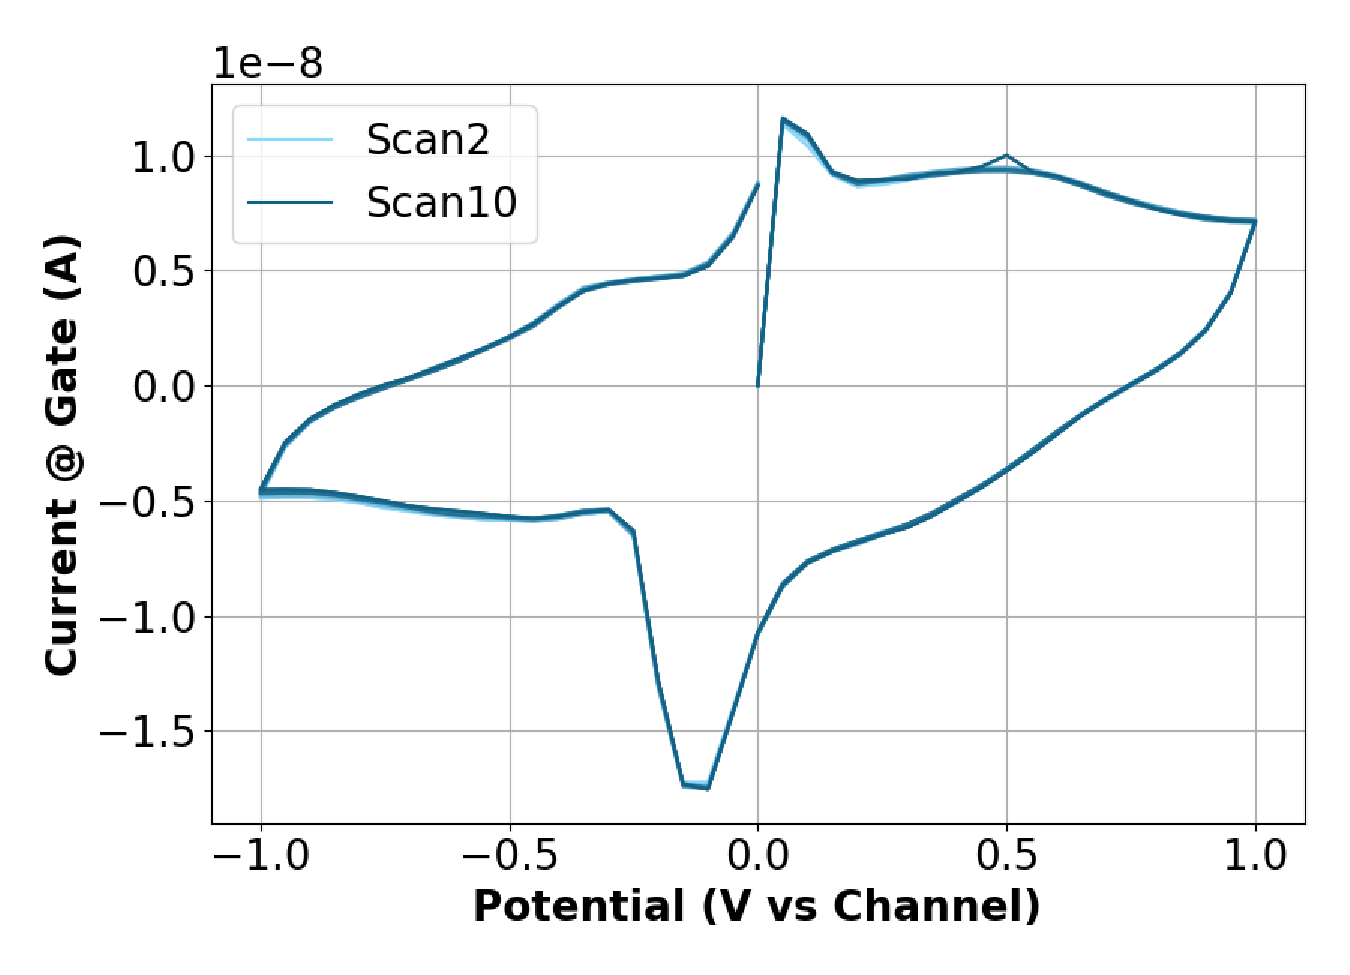
\includegraphics[width=6cm]{Images/pdf/CV_photo.pdf} }}
    \caption[Performance of solid-OECT with photolithographed SSE]{A) Micrograph of patterned device before and after application of SSE, B) transfer characteristics at $V_{DS}$ of -0.1 V. And representative C) Bode plot obtained by EIS and C) redox behavior between Au/p(g3T2-T) and SSE using CV.}
    \label{fig:photoSSE}
\end{figure}
%Photo I am using D5

The channel and volumetric capacitance shows a clear increase compared to drop-casted SSE. %, this may be due to the lack of device crosstalk
However, CV graphs exhibit two different behaviors, with oxidation and reduction potentials falling into the ranges represented in Table \ref{tab:photofom}, suggesting that some oxidation is still perceived in most devices.

\begin{table}[ht]
\centering
\caption{Parameters extracted from the characterization of photopatterned SSE OECT}
\begin{tabular}{l|c||l|c}
Parameters & Value & Parameters & Value \\\hline \hline
V$_{Th,forward}$ [V] & -0.08 $\pm$ 0.05 & V$_{Th,backward}$ [V] & -0.09 $\pm$ 0.04\\
& & &\\[-1em]
C$_{channel}$ [nF] & 81.6 & C* [Fcm$^{-3}$] & 87.7 \\
%C$_{channel}$ [nF] & 58.7 $\pm$ 24.4 & C* [Fcm$^{-3}$] & 63.1 $\pm$ 26.2 \\
& & &\\[-1em]
V$_{ox}$ [V] & 0.04, 0.34  & V$_{red}$ [V] & -0.1, -0.2 \\
& & &\\[-1em]
|g$_{m,max}$| [mS] &  &  &\\\hline
\end{tabular}
\label{tab:photofom}
\end{table}

Upon exposure to ambient environment, measurements revealed depletion-mode devices with a positive gate bias. Suggesting that, unlike drop-casted SSE, photopatterned SSE does not provides sufficient ``shielding'' to prevent oxidation of p(g3T2-T).

Figures\\
Table with parameters.

\newpage
\subsubsection{OECT with Inkjet-Printed SSE}%Solid-State Electrolyte}
%The Ag/AgCl gate electrode’s work function is reasonably constant, the work function of an OMIEC gate electrode however may vary depending on its processing history and redox reactions with other species present in the electrolyte (e.g. molecular oxygen).28 Applying VGS only determines the potential difference between the gate and channel but does not control the potentials of either electrode (hence the position of the Fermi level) with respect to a reference. This leads to many challenges in operating an OECT with OMIEC gate electrodes \cite{tanOperationMechanismOrganic2021}.

Despite high yields in the patterning process, only four devices were successfully printed. Out of which, only one was fully operational, and it will be used in this analysis.

The process of printing SSE on top of the patterned gate and channel p(g3T2-T) remains a challenge. The process takes approximately 2 hours per sample under ambient conditions. Efforts were made to set the printing parameters using a different sample while exposing our device to high temperatures and ethanol rinsing to revert oxidation. Unfortunately, the resulted device still exhibited signs of oxidation.

\begin{figure}[ht]
    \centering
    \subfloat[]{{\includegraphics[width=6cm]{Images/pdf/und_ink.pdf} }}
    \subfloat[]{{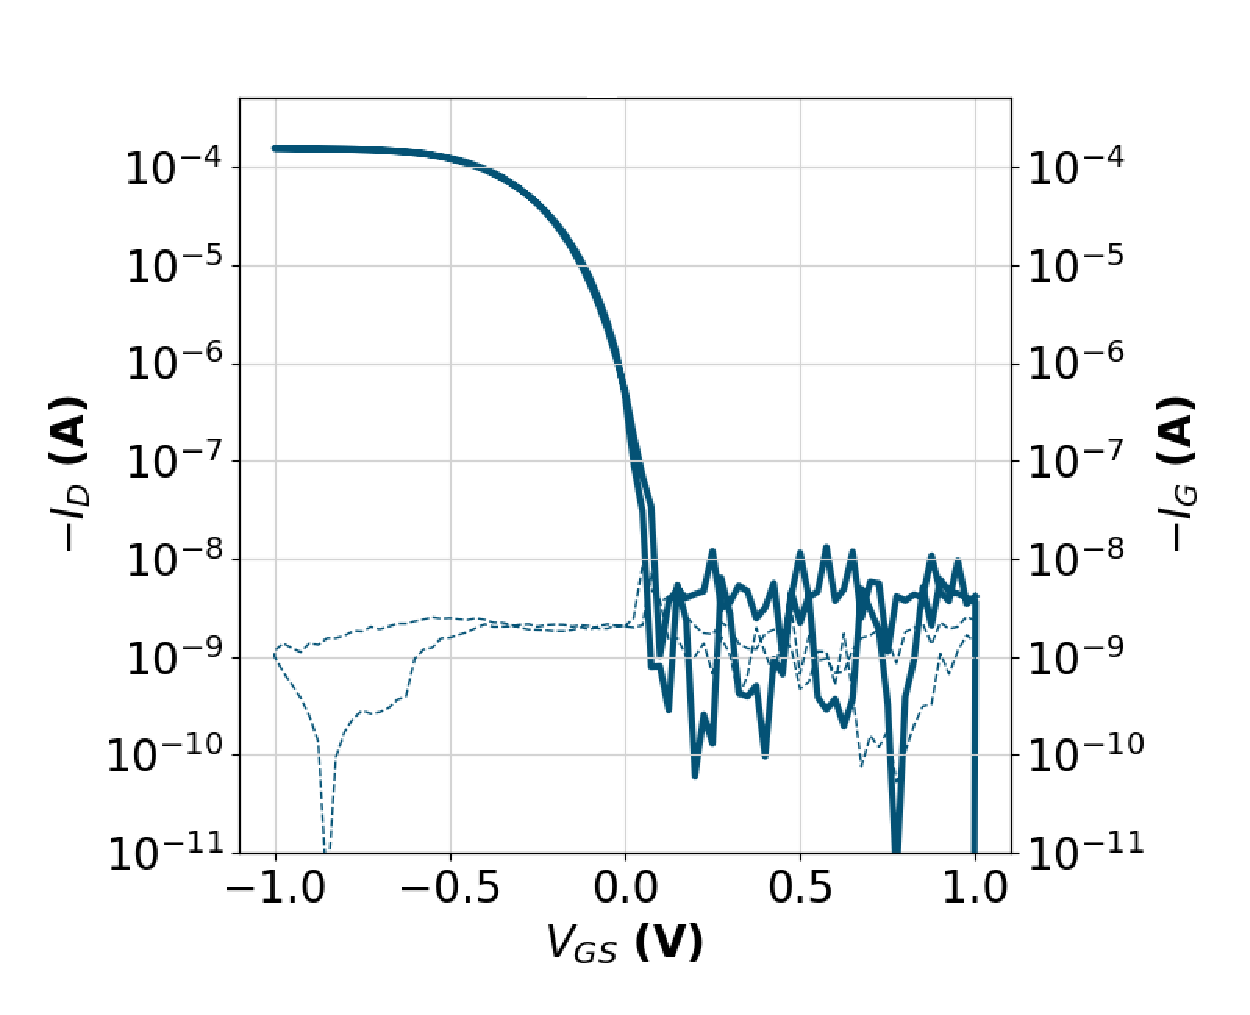
\includegraphics[width=6cm]{Images/pdf/transfer_ink.pdf} }}
    \qquad
    \subfloat[]{{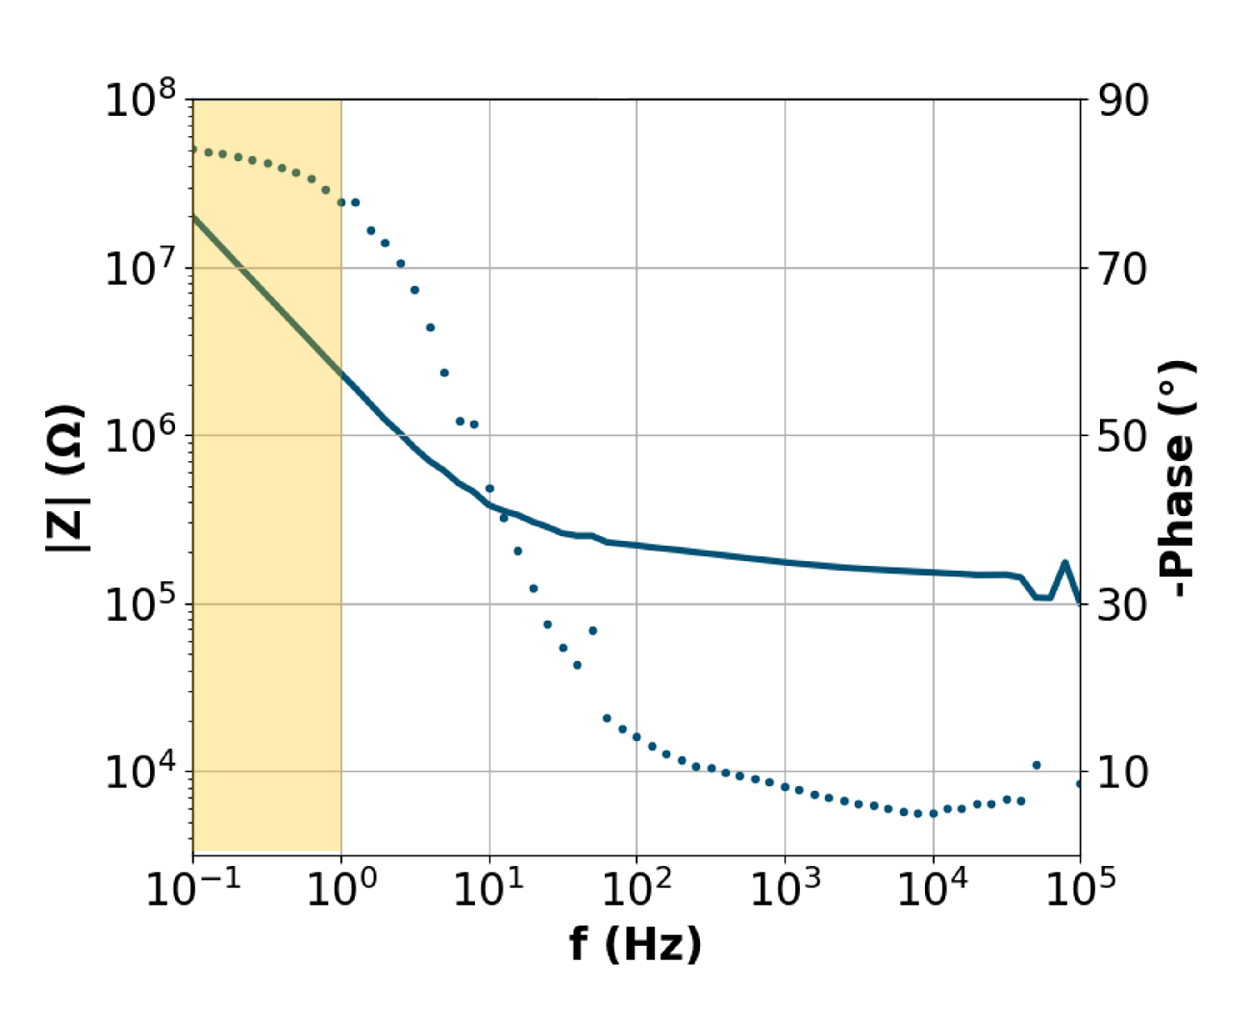
\includegraphics[width=6cm]{Images/pdf/EIS_ink.pdf} }}
    \subfloat[]{{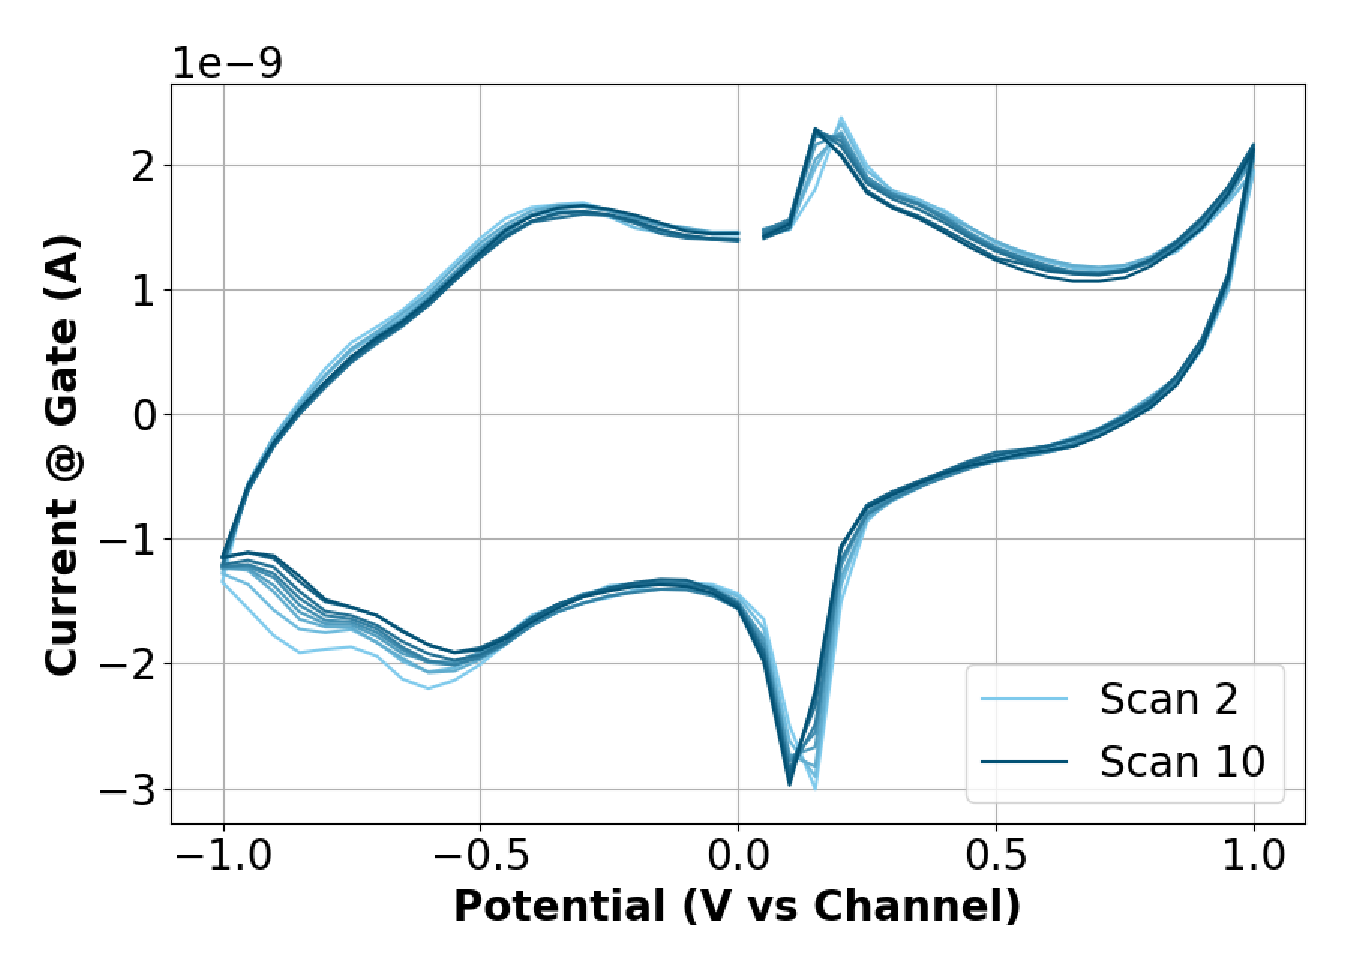
\includegraphics[width=6cm]{Images/pdf/CV_ink.pdf} }}
    \caption[Performance of solid-OECT with printed SSE]{A) Micrograph of patterned device with printed SSE, B) transfer characteristics at $V_{DS}$ of -0.1 V. C) Bode plot obtained by EIS and C) redox behavior between Au/p(g3T2-T) and SSE using CV.}
    \label{fig:printedSSE}
\end{figure}
%printed i only have one, U5



\begin{table}[ht]
\centering
\caption{Parameters extracted from the characterization of printed SSE OECT}
\begin{tabular}{l|c||l|c}
Parameters & Value & Parameters & Value \\\hline \hline
V$_{Th}$ [V] &  0.13 & |g$_{m,max}$| [mS] & \\
& & &\\[-1em]
C$_{channel}$ U5[nF] & 85.3 & C* [Fcm$^{-3}$] & 91.6 \\
& & &\\[-1em]
V$_{ox}$ [V] &  & V$_{red}$ [V] &  \\\hline
C$_{channel}$ D6 [nF] & 289 & C* [Fcm$^{-3}$] & 311 \\\hline
\end{tabular}
\label{tab:printedfom}
\end{table}


\subsection{Solid-OECTs using Doped-p(g3T2-T)} \label{dopedOECTs}

\subsubsection{Channel conductivity}
The channel conductivity was monitored using SSE precursor after exposure, and the $I_{D}$ no longer decreased but maintained its initial values of ... mS, as seen in Figure ...

Different doping levels were intended to be studied in this section. However, only 5 mg/mL of F$_{6}$TCNNQ showed doping homogeneity that would allow a fair comparison. Figure ... shows irregularities in the doping when using 10 and 15 mg/mL of dopant concentration. Acetonitrile solvent was unable to correctly dissolve this dopant, and achieving higher dopant concentration that may led to depletion-mode OECTs was not possible.

\subsubsection{Solid-OECT performance}

The adhesion promoter used for undoped p(g3T2-T) could not be used for doped species since it will remove dopants during the application steps. An alkaline-based adhesion promoter would be needed, which required additional experiments to test its effectiveness. Therefore no promoter was used, and low yields in printing were expected despite the high yields in patterning.

Eight operational devices were obtained. However, only one exhibited a capacitive behavior that allowed for transfer characteristics, and it will be used in this analysis. Transfer characteristics, EIS and CV measurements are shown in Figure \ref{fig:dopedSSE}, and the calculated parameters are exhibited in Table \ref{tab:dopedfom}.

%% U7
\begin{figure}[ht]
    \centering
    \subfloat[]{{\includegraphics[width=6cm]{Images/pdf/doped_ink.pdf} }}
    \subfloat[]{{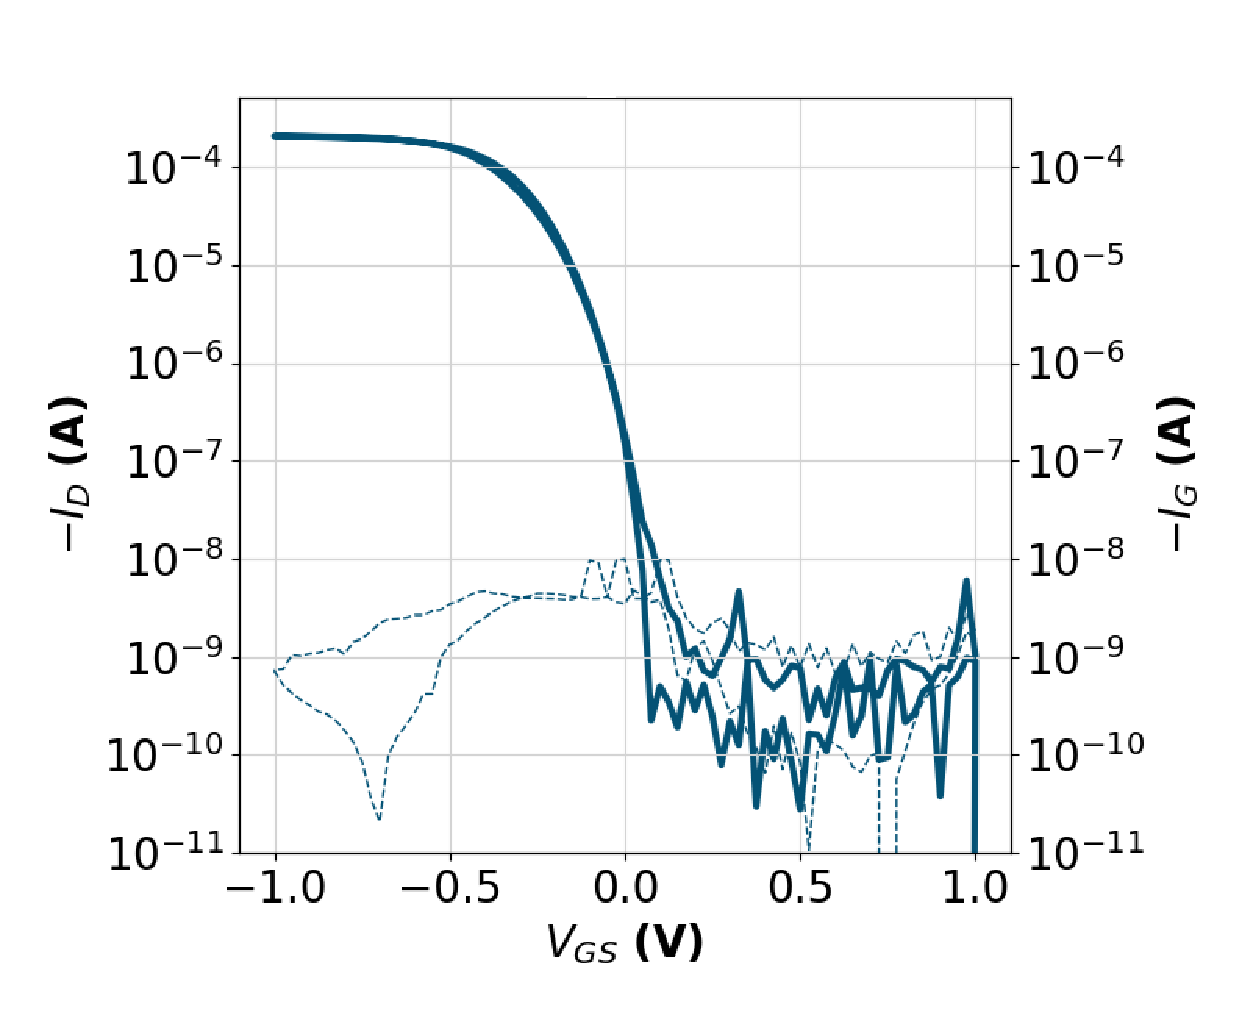
\includegraphics[width=6cm]{Images/pdf/transfer_doped.pdf} }}
    \qquad
    \subfloat[]{{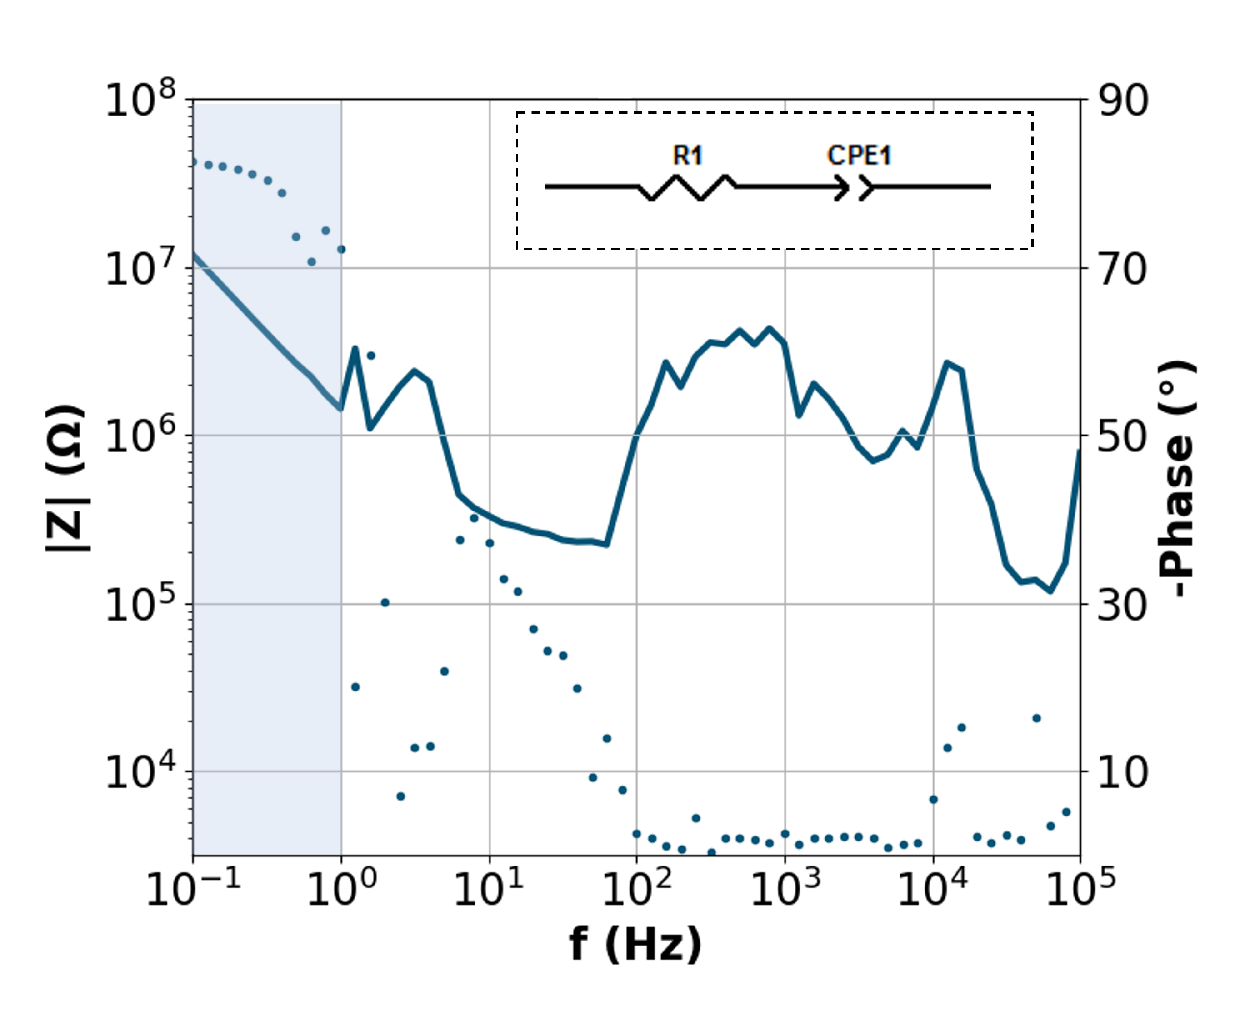
\includegraphics[width=6cm]{Images/pdf/EIS_doped.pdf} }}
    \subfloat[]{{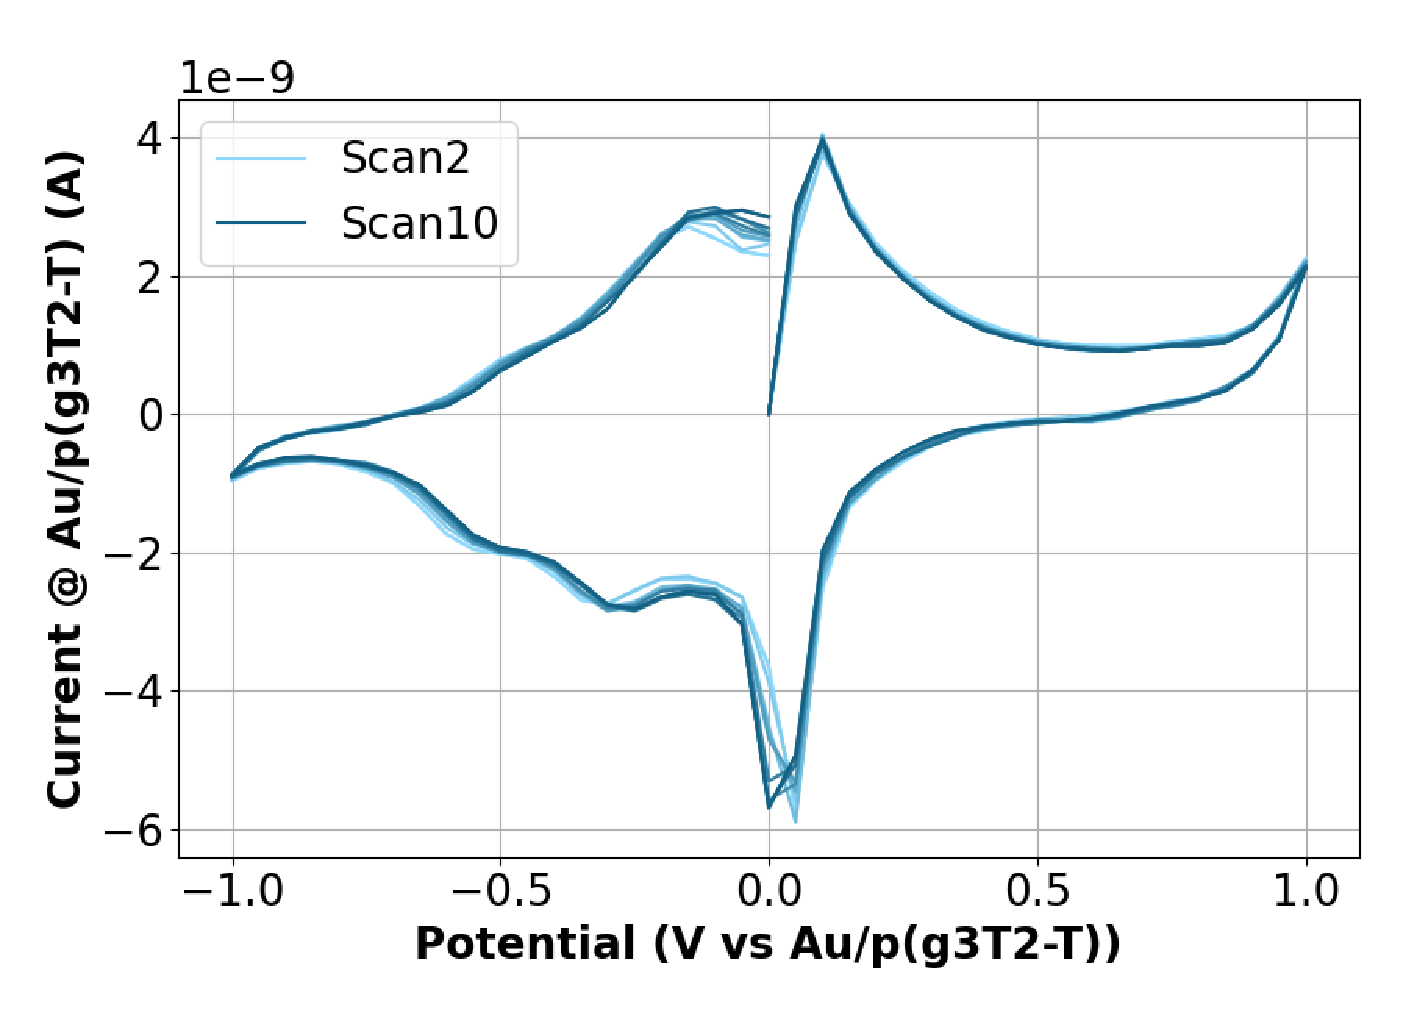
\includegraphics[width=6cm]{Images/pdf/CV_doped.pdf} }}
    \caption[Performance of solid-OECT with doped-p(g3T2-T)]{A) Micrograph of patterned device with printed SSE, B) transfer characteristics at $V_{DS}$ of -0.1 V. C) Bode plot obtained by EIS and C) redox behavior between Au/p(g3T2-T) and SSE using CV.}
    \label{fig:dopedSSE}
\end{figure}

\begin{table}[ht]
\centering
\caption{Parameters extracted from the characterization of doped-p(g3T2-T) OECT}
\begin{tabular}{l|c||l|c}
Parameters & Value & Parameters & Value \\\hline \hline
V$_{Th}$ [V] & -0.1 & |g$_{m,max}$| [mS] & \\
C$_{channel}$ [nF] & 130 & C* [Fcm$^{-3}$] &  140 \\
V$_{ox}$ [V] & 0.1 & V$_{red}$ [V] & 0.0 \\\hline
\end{tabular}
\label{tab:dopedfom}
\end{table}

%Achieving effective charge transfer between the analyte and OMIEC requires appropriate alignment of the electrochemical potential of electrons on the OMIEC electrode and the redox specie. Failure to do so may result in the subsequent transfer of charges to other redox-active sinks in the environment, leading to undesirable side reactions and products that may interfere with the OMIEC’s operation. Electrons flow from a region of higher to lower electrochemical potential. Hence, achieving electron transfer from redox-active species to the OMIEC requires the latter to have a deep LUMO (high electron affinity) \cite{tanMixedIonicElectronic2022} %paper


\newpage

\subsection{Threshold Voltage Shift} \label{vth_shift}

%\section{Conclusion}
%\lipsum[86-88]

%%% Local Variables: 
%%% mode: latex
%%% TeX-master: "thesis"
%%% End: 
